\documentclass[12pt]{article}

\usepackage[english]{babel}
\usepackage{graphicx}
\usepackage{csquotes}
\usepackage[margin=2cm]{geometry}

\usepackage{amsmath,amsfonts,amssymb,amsthm, bm}
\usepackage{hyperref}               % Hyperlinks
\usepackage{totcount}               % Last value of counter
\usepackage{pgffor}                 % For loop
\usepackage[dvipsnames]{xcolor}     % Colors
\usepackage{indentfirst}            % Indent paragraphs
\usepackage{caption}
\usepackage{subcaption}
\usepackage{multirow}
\usepackage{array}
\usepackage{algorithm}
\usepackage{algorithmicx}
\usepackage{algpseudocode}
\usepackage[T1]{fontenc}
\usepackage{tablefootnote}
\usepackage[skip=5pt plus1pt, indent=40pt]{parskip}

\usepackage[sorting=none]{biblatex}               % Bibliography
\bibliography{resources/bibliography}
% \addbibresource{resources/bibliography.bib} %Import the bibliography file
\usepackage[nottoc,numbib]{tocbibind}

\graphicspath{{resources/images}}

\hypersetup{
    colorlinks,
    citecolor=black,
    filecolor=black,
    linkcolor=black,
    urlcolor=Blue
}


% see https://tex.stackexchange.com/a/165688, counters adapted

\newtotcounter{countWarnings}
\setcounter{countWarnings}{0}
\newcommand{\mywarningformat}[1]{\textit{\color{red}#1}}
\newcommand*{\mywarning}[1]{
    \addtocounter{countWarnings}{1}
    \hypertarget{warning\thecountWarnings}{}
    \mywarningformat{#1}
}
\newcommand{\mylistwarnings}[1]{
    \foreach \i in {1,...,\totvalue{countWarnings}} {
        #1\hyperlink{warning\i}{\texttt{Warning} No.\i}
    }
}

\numberwithin{equation}{section}
\numberwithin{figure}{section}
\numberwithin{table}{section}

\DeclareCaptionType{captionnable}[][]
\newcommand{\equationcaption}[1]{\caption*{Equation \theequation: #1}}

\renewcommand{\labelitemi}{--}

\graphicspath{ {./resources/images/} }







\begin{document}%\layout

\begin{titlepage}

    \begin{center}

    \begin{figure}[t]
        
\includegraphics[width=0.7\textwidth]{uliege-logo-couleurs-300.jpg}
        \centering
    \end{figure}
    \large University of Liège - School of Engineering and Computer Science\\[0.5cm]

    \rule{\linewidth}{0.5mm}\\[0.2cm]

    \textsc{\Large MASTER'S THESIS}\\[0.5cm]

    \textbf{\LARGE Improving the simulation of variable renewable energy in the MEDEAS integrated assessment model}

        \rule{\linewidth}{0.5mm}\\[2cm]

        Master's thesis completed in order to obtain the degree of Master of Science in Computer Science Engineering by \textsc{Straet} François\\[4cm]

    \end{center}

    \textbf{Supervisor:}

    Prof. S. Quoilin\\[1.5cm]
    

    \center

    Academic year 2022-2023

\end{titlepage}


\pagenumbering{roman} 

\section*{Acknowledgements}

I would like to thank professor Quoilin first, for his mentoring during this thesis and his advices. Then Jade, for her collaboration on the linkings between the created model and MEDEAS.

Computational resources have been provided by the Consortium des Équipements de Calcul Intensif (CÉCI), funded by the Fonds de la Recherche Scientifique de Belgique (F.R.S.-FNRS) under Grant No. 2.5020.11 and by the Walloon Region. I am also grateful to the cluster administrator, M. Collignon, for his patience and valuable advices.

Thanks should also go to my mother, and everyone to which I talked about my thesis, what sometimes led me to get a new perspective on the work as I had to explain it in a new, concise and understandable way.

\newpage

\section*{Abstract}

This master thesis explores the use of a surrogate model to achieve the integration of electricity network constraints into integrated assessment models, that attempt to predict the evolution of the main features of the society, including economic, demographic, climatic and energy factors.

Tools were developped to run Dispa-SET, a dispatch model for the European electricity network, to build a dataset of simulations on adequate sample points. This dataset is then used to train the surrogate model using appropriate machine learning methods. Finally, this model is integrated into the MEDEAS IAM, connecting their variables in a meaningful way, and the resulting model is run for different scenarios.

Results show that integrating the model in MEDEAS leads to a lower prediction of the production of variable renewable energy sources compared to the initial MEDEAS output.

\vspace{1cm}
Keywords: surrogate model, Dispa-SET, MEDEAS, machine learning, VRES

\newpage

\tableofcontents

\subsection*{Warnings}

I have \total{countWarnings} warnings:
\begin{itemize}
    \mylistwarnings{\item}
\end{itemize}

\newpage

\section*{Keywords}

\addcontentsline{toc}{section}{Keywords}

\begin{table}[h!]
    \begin{tabular}{p{3cm} p{8cm}}
        AF & Availability factor \\
        CF & Capacity factor \\
        DLL & Dynamically loaded library \\
        LP & Linear programming \\
        LHS & Latin hypercube sampling \\
        MILP & Mixed integer linear programming \\
        MTS & Mid-term scheduling \\
        P2H & Power to heat \\
        RES & Renewable energy sources \\
        VRES & Variable renewable energy sources \\
    \end{tabular}
\end{table}

\newpage


\pagenumbering{arabic}

\section{Introduction}

Our societies run on energy. Energy is required to power pretty much whatever we do and need. Fossil fuels provided us with relatively easy to access, store and use energy for decades, bringing a solution to a problem.

Now, the awareness of the climate change, mostly caused by the release of large amounts of greenhouse gases, among them carbon dioxyde, produced by the combustion of these fossil fuels, is a game-changer. In order to acheive set targets in terms of climate evolution, bounds on carbon emissions have been defined, and therefore limiting the prevously endless source of energy that were fossil fuels in the very long run.

The solutions to compensate for the lacking energy generation, that from now on should not originate from fossil resources, are renewable energy sources. These refer to every energy generation technique originating from a renewable source, such as the sun, the wind and the rivers. However, the creation of these units may not be completely renewable in itself, for example, the photovoltaic cells necessary for the exploitation of the incoming solar energy are pretty difficult to recycle, making them rely on specific materials that are not obtainable renewably. Still, their use on a complete lifetime, and increasing capabilities in recycling, pays off the invesment made at their construction.

In this context, a significant increase in the energy produced from such energy sources is to be expected, in particular, from:
\begin{itemize}
    \item the sun, through photovoltaic panels,
    \item the wind, through on-shore and off-shore wind turbines, and
    \item rivers, through hydroelectric dams.
\end{itemize}

The third one, due to its dependency on the geographic context, will however not expand foerever, as there are not illimited spots to build such dams.

One thus falls back to photovoltaic and wind energy, but both have a major, trivial drawback: they rely on the sun and the wind, respectively. And this becomes a huge deal, because the amount of energy that can be generated by exploiting these is variable, hence their designation as variable renewable energy sources, or VRES.

It is to be mentioned that these variabilities comprise some predictability, for example, there is on average more photovoltaic production potential during summer. On a daily scale as well, with the day night cycle. Weather forecasts can also be taken advantage of in order to predict wind turbines' production.

The larger variability of the power output of VRES causes a problem, because modern electrical system is dictated by consumers' demand. And to do so, electricity generators are dispatched in real-time, so that the production always matches the demand on the network. This technique works because the concerned power plants can be started and shut down on demand, almost at any time. With VRES, this assumption drops, as one cannot start an extra wind turbine if there is no wind, nor use a photovoltaic panel during the night.

\subsection{Flexibility assessment in energy system models}

As explained before, higher shares of VRES in the electricity production mix create the additional challenge, that is the handling of the partlially predictable variability of wind and sun energy. 

This handling requires a larger flexibility of the electrical system, that is, a better ability to adapt to changes in the demand and supply, either expected or not \cite{irena}.

To improve the flexibility of an existing power system, some mechanisms already exists.

\begin{itemize}
    \item Use of the regular dispatchable energy production plants to mitigate the energy not produced from VRES. Depending on the plant characteristics, it may be difficult to address short term drops in production, as there is some start up time required \cite{flexibility-storage-planning}.
    \item Large interconnected electricity networks, that are able to smooth the VRES power output. There may be not enough sun in some region, creating a deficit, while there is too much in the neighboring country. By connecting them, the overproduction will compensate the unerproduction of the other \cite{flexibility-connection}.
    \item Energy storage facilities. Of course, storing the produced energy for later use is an easy way to account for the intermittency of the production. Typically, storing solar energy during day time to be used in the night. These technologies include pumped hydro-storage, batteries, compressed air. While pumped hydro-storage units are the most common, their very limited expansion options make them unlikely to grow in the future \cite{flexibility-demdandside-forecasts-storage}.
    \item Acting on the demand, in the extent that it can change its shape by promoting policies to the end users. Such policies focus on flattening the daily demand curve, facilitating the energy production dispatch. Typically, asking to delay greedy devices like dishwashers until night, where the overall demand is lower. But it may concern other domains, such as electric vehicles charge, heating and cooling etc \cite{flexibility-demdandside-forecasts-storage}.
\end{itemize}

The two main consequences of insufficiently flexible energy systems are curtailment, when there is too much energy produced, and load shedding, when there is not enough electricity to satisfy the demand. In case of load shedding, parts of the grid may be entirely shut down.

\subsubsection{Literature review}

Similar work has been done by Parrado-Hernando et al. in \cite{Hernando2022}, that aims at "capturing features of hourly-resolution energy models". The methodology used to acquire the data presents two downsides that are adressed in this work.

First, the inputs of the energy model are handled as discrete variable, and simulation have been run using all possible combination for these values. This can be seen in some of their figures, where the data points seem to follow some lines. While it does not invalidate the process, this creates a bias in the repartition of the data. Second, linear approximation are used to fit the data obtained. Admittedly, this is identified as a limitation of the work.

To palliate these, the input space will be tackled as a continuous domain for the design of experiment, and other machine learning technique will be considered as to candidates for the creation of the surrogate model.

\subsection{Short-term dispatch models}

There exists tools built in order to assess the behaviour of large electrical systems, that are subject to higher share of VRES. These tools typically aims at predicting the electricity flows, dispatching available power plants in order to match the production to the demand. And from there on, some higher level metrics can be computed, and in particular, we will be interested by:
\begin{itemize}
    \item the curtailment, that is, the energy produced in excess while the electricty demand was already met, that end up wasted, and
    \item the lost load, that is, the energy that could not be produced, hence some demand could not be served.
\end{itemize}

Among these tools, the Dispa-SET model will be considered in this work. Dispa-SET is open-source, and focused on balancing problem in the European grid specifically.

This model is formulated in linear programming, that is, a set of linear constraints are defined and an objective function is given. The solver inputs both of these and computes the parameters values that maximize the objective function while matching the constraints.

\subsection{Integrated assessment models}

On another level, integrated assessment models (IAM) aim at estimating the evolution of large, intricated systems involving a lot of different interconnected areas and actors. These are most often multidisciplinary and require a lot of modelling choices.

In particular, some IAM attempt to model the evolution of the whole society, from a socio-economical perspective, including environmental aspects and energy concerns.

In this subset of IAMs, the MEDEAS model is chosen for this work, being open-source as well and providing a EU-specific model.

MEDEAS is expressed in terms of systems dynamics, that is, the evolution of the state of the simulation is computed as a function of its current state. And this comes down to solving a set of differential equations.

\subsection{Model linking}

Due to computational constrain, IAMs often have a pretty low level of temporal, or spacial accuracy \cite{linkings-stuff}. This is not the case for dispatch models, that carry out more extensive simulations. Therefore, it is meaningful to link two of these models together, as the IAM would benefit from the better accuracy of the energy models. 
% As MEDEAS does not extensively simulates the dispatch of power plants units for the sake of its estimate of the curtailment and lost load, that are used in the model, its estimations of these values are not as precise as those computed by Dispa-SET. Therefore, MEDEAS would benefit from a linking between the two models.

An high-level illustration of the positionw of MEDEAS and Dispa-SET on the timescale is provided on Figure \ref{fig:dispaset-medeas-timescale} \cite{dispaset}.

\begin{figure}[h]
    \centering
    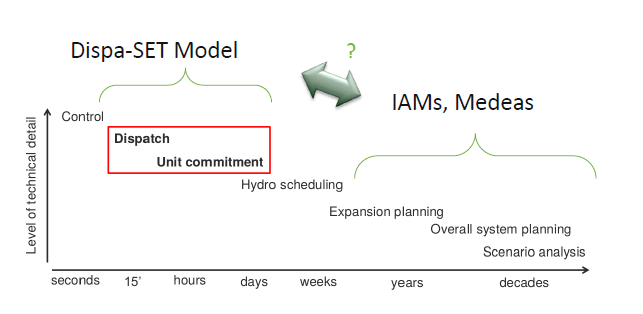
\includegraphics[width=0.8\textwidth]{resources/images/dispaset-medeas-timescale.png}
    \caption{An illustration of where Dispa-SET and MEDEAS operate on the timescale}
    \label{fig:dispaset-medeas-timescale}
\end{figure}

\subsubsection{Linking types}

There are several strategies that may be used in order to link two models together \cite{linkings-stuff}.

\begin{itemize}
    \item Soft linking: the models communicate between each other. This communication may be uni-directional or bi-directional. Both of the models are run iteratively, thus keeping their separate efficiencies in the same order of magnitude. However, the iteration lead to low overall speed, and convergence is not guaranteed.
    \item Hard linking: the models are combined into a single, unified mathematical formulation. This newly created model can then be solved all at once. This approach is burdened by higher computational costs and lower chance of feasibility.
\end{itemize}

These linking types are illustrated on Figure \ref{fig:linking-types}.

\begin{figure}[h]
    \centering
    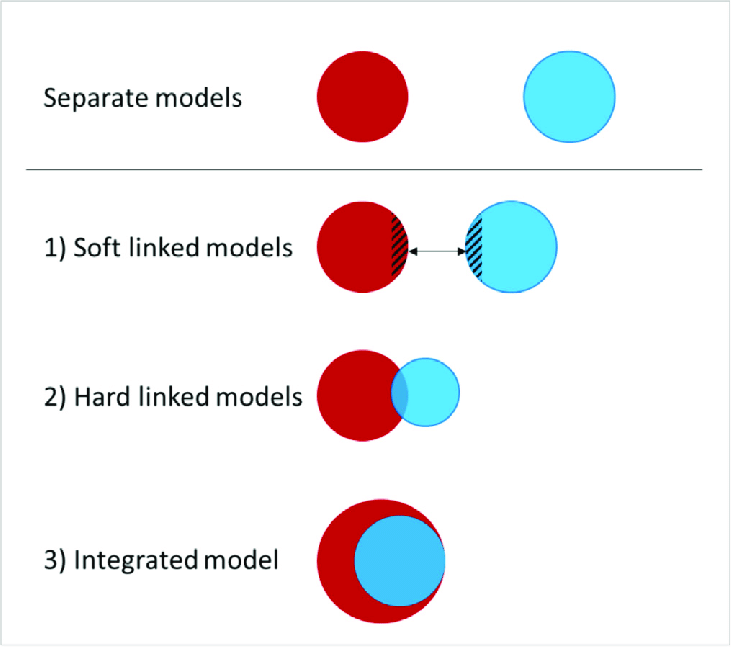
\includegraphics[width=0.4\textwidth]{resources/images/hybrid_model_variants.png}
    \caption{Illustration of the different linking methods \cite{hybrid_models}.}
    \label{fig:linking-types}
\end{figure}

One may also add model integration, consisting in completely embedding a model into the other. But this is not tractable in this setting, and would also requires compatible model formulations, as explained below.

In this case, hard linking is not possible due to the different formulations of Dispa-SET, in linear programming, and MEDEAS, in differential equations.

We also dismiss the soft linking strategy because of its slowness, and absence of convergence guarantee.

\subsubsection{Surrogate models}

The linking technique explored in this work is the surrogate model. In this case, an approximation of the Dispa-SET dispatch model will be integrated in the MEDEAS IAM. 

The idea behind surrogate models is simple. First, a fast, easy-to use approximation of the model is made, then it its completely integrated in the other model. In this case, the relevant outputs of the Dispa-SET model will be approximated from relevant inputs regarding MEDEAS, then the approximator will be integrated in the model.

The soft-linking approach has already been explored \cite{Brinkerink2022-softlink}, \cite{DEane2012-softlink}, and the hard-linking remains the hardest to investigate, notably due to incompatible formulations. Surrogate models are still unexplored and are of great interest for this use case.

As the combination of the model will use an approximation, this appriximation being fast will not burden the computations of the IAM, hence keeping it efficient.

\subsection{This work}

\subsubsection{Objective}

This master's thesis is dedicated to the integration of the flexibility constraints, the Dispa-SET surrogate model, into the MEDEAS model, being less precise on the matter. This includes the creation of a proper dataset, the definition, training and integration of the surrogate model into MEDEAS.

% \subsubsection{Methodology}

% To do so, adequate design of experiment will be conducted on well-chosen, continuous, input parameters, that will in fine be the surrogate model input features. This will give us a set of input points where a Dispa-SET run will be made, to create a training sample, and the samples are grouped into a single dataset.

% Once this dataset is built, one can then choose and train a model to become the surrogate model on it. The model is chosen after a short assessment of candidate machine learning options.

% When the model will be available, it will then be usable from inside MEDEAS, where some connection will have to be drawn between the variables that are already present in the model, and the surrogate model actual input and output features.

% Finally, the resulting adapted MEDEAS model will be run, and observations and criticisms will be made.

\subsubsection{Contributions}

This works follows what was started by another student, Carla Vidal, that went until the surrogate model training, included. Given that improvements where implemented in Dispa-SET since then, the runs had to be re-done. However, there were no easy to use scripts to set up the simulation files etc., so that is has been chosen to write new ones.

Furthermore, the present thesis also considers other machine learning algorithms, although the same choice of neural networks is made, this time based on better performance compared to the other options.

Another student, Jade Paris, was in charge of the linking of the surrogate model, given as a functions of some inputs variables into the MEDEAS model, and its actual use and runs of MEDEAS with the surrogate model integrated.

This work constisted in:
\begin{itemize}
    \item The writing of easy-to-use scripts to run Dispa-SET on those experiments
    \item The efinition and implementation of an adequate machine learning model (neural net), and training
    \item The integration the model in MEDEAS, by writing a C++ external function library for Vensim, or by inserting it into the PySD model of MEDEAS directly in python
    \item Runs and analysis of the improved MEDEAS model
\end{itemize}

All the produced work, and necessary data is available on the online github repository at the following address: \href{https://github.com/Rayerdyne/master-thesis}{https://github.com/Rayerdyne/master-thesis}.

\subsubsection{Outline}

This document is organized into seven main sections. The second section presents an in-depth description of the Dispa-SET model, along with the tools employed within its framework. Following this, the third section provides a detailed account of the MEDEAS model, outlining its underlying principles and the broader framework in which it operates.

To facilitate the successful integration of models, the fourth section outlines the process of data generation. This encompasses a complete overview of the methodologies employed to produce the necessary training data, the design of experiments and the execution of Dispa-SET runs.

Subsequently, the fifth section characterizes the surrogate model, offering a comprehensive description of its design. The section further expounds on the training and validation processes undertaken to ensure the surrogate model aligns accurately with the main models' outcomes.

The sixth section then shifts the focus to the crucial process of integrating the surrogate model into MEDEAS. A step-by-step description is provided, elucidating how the surrogate model becomes an integral component of the broader MEDEAS framework, and how it interacts with the existing models.

Finally, the document concludes in the seventh section, offering a comprehensive summary of the resulting model and outcomes. This concluding section also identifies any limitations and outlining future areas of research for further enhancements. 

% This document is structured as follows:

% \begin{enumerate}
%     \item \textbf{The Dispa-SET model}: description of the Dispa-SET model and tools
%     \item \textbf{The MEDEAS model}: description of the MEDEAS model and framework
%     \item \textbf{Data generation}: description of the complete process to generate the training data, that is, the design of experiments and the Dispa-SET runs
%     \item \textbf{The surrogate model}: definition of the surrogate model, training and validation
%     \item \textbf{Integration}: description of the process of integrating a model into MEDEAS
%     \item \textbf{Analysis}: the analysis of the runs of MEDEAS with the integrated surrogate model
%     \item \textbf{Conclusions}
% \end{enumerate}

\section{Chapter1}

Hello world!
\section{Data generation}

\subsection{Overview}

This section aims at describing the process that lead to the creation of the dataset, required in order to train the neural network model.

First, an input space is defined, on which will properly select points to form the dataset features. Then, computationally expensive simulation will be run on these points to obtain the desired predicted features for this dataset.

This dataset will afterwards be used to train the surrogate model on \cite{surrogate_model}.

\subsection{Preparatory work}

As stated earlier, this setting only considers the european power system in Dispa-SET, then to create and validate our surrogate model. Each simulation is run over a period of 2019.

\subsubsection{Unit groupings}
In this context, the precise technology and fuel types of each plant is not relevant, as they won't influence the input features of our dataset. Hence, the units are grouped into five categories: flexible units, slow units, storage units, PV units and wind units.

IRENA \cite{irena} describes flexible units as "units that can ramp up and down quickly, have a low minimum operating level and fast start-up and shutdown times", what criterion will be used to separate regular units into the slow and flexible units. This criterion is presented in Table \ref{table:flex-vs-slow-unit}.

\begin{table}[h!]
    \centering
	\begin{tabular}{|l | l | p{8cm}|}
		\hline
		Units & Fuel & Condition \\
		\hline
		$Flex_{units}$ & \multirow{2}{3cm}{GAS, HRD, OIL, BIO, LIG, PEA, NUC, GEO} & $PartLoadMin<0.5$ and $TimeUpMin<5$ and $RampUpRate>0.01$\\ \cline{1-1} \cline{3-3}
		$Slow_{units}$ &  & $PartLoadMin\geq 0.5$ or $TimeUpMin \geq 5$ or $RampUpRate\leq 0.01$\\
		\hline
	\end{tabular}
	\caption{Flexible and slow units classification criterion}
	\label{table:flex-vs-slow-unit}
\end{table}

Refer to Tables \ref{table:technologies-eu} and \ref{table:fuels-eu} for their names.

One also has to consider the limit to the number of hydroelectric units that are possible to build given a geographical area. Given that EU is already almost at saturation, stationary batteries are considered, among other energy storage technology (e.g. compressed air, electric vehicles' battery grid).

As for the other groups, they can be simply described with technology-fuel pairs as follows:
\begin{itemize}
    \item $Storage_{units}$ with (OTH, BATS)
    \item $PV_{units}$ with (SUN, PHOT)
    \item $Wind_{units}$ with either (WIN, WTON) or (WIN, WTOF), the latter not being considered in this work
\end{itemize}

\subsubsection{Parameters estimates}

The availability factors of PHOT and WTON are also required, as well as the peak load. These values are computed from the reference simulation (2019), and are shown in Table \ref{table:param-values}.

\mywarning{needs check}

\begin{table}[h]
    \centering
    \begin{tabular}{|l c c|}
        \hline
        Variable     & Value  & Units \\ \hline
        $AF_{PV}$    & 0.1313 & \%    \\
        $AF_{WTON}$  & 0.2604 & \%    \\
        $PeakLoad$   & 440929 & MW    \\ \hline
    \end{tabular}
    \caption{Values of availability factors and peak load}
    \label{table:param-values}
\end{table}

\subsection{Design space}

\subsubsection{Shape}

The first necessary step in order to select our data points for our dataset, is to define the space in which we will sample them. In our case, this space will be the product of 6 ranges, that is a 6 dimensional hypercube. 

One may argue that some areas of this hypercube, typically around the vertices, will be extremely unlikely to happen in a real setting. More precisely, as this cube will be the input space of the surrogate model that will be connected to another model, it may be suitable to prune the areas of the cube that will never be reached. Indeed, if we know that some areas will never be queried, there is no use covering them.

Furthermore, assuming we would obtain the exact space of possible queries, this space is not likely to be close to some common shape (hypercube, hyperball or combination). Given that most of the design of experiments techniques assume these kinds of space, a mapping would be needed to benefit from the better sampling strategies. Such a mapping would be pretty complex to develop.

More importantly, the cost of being more general than strictly required is small, mainly consisting of a slightly larger surrogate model (in this specific case, a larger neural network), and a larger dataset.

For these reasons, an hypercube will be used.

\subsubsection{Variables}

The six adimensional variables, corresponding to a dimension, are described below, with their given range.

The notation $PowerCap_{x}$ refers to the maximum power output of all the units in $x$. See Table \ref{table:param-values} for the values of the AF and peak load value.

\begin{enumerate}
    \item \textbf{CapacityRatio [$\cdot$]}
    
    Ratio of the maximum production over the maximum demand.
    \begin{equation}
        CapacityRatio  = \frac{PowerCap_{flex units}+Power Cap_{slow units}+PowerCap_{storage units}}{Peak Load}
    \end{equation}

    \item \textbf{ShareFlexibility [$\cdot$]}
    
    Share of the units that are flexible.
    \begin{equation}
        {Share_{flex}}=\frac{PowerCap_{flex units}}{Power Cap_{flex units}+PowerCap_{slow units}}	
    \end{equation}

    \item \textbf{ShareStorage [$\cdot$]}
    
    Ratio of the maximum power output of all storage units over the maximum demand.
    \begin{equation}
        {Share_{storage}}=\frac{PowerCap_{storage units}}{Peak Load}	
    \end{equation}

    \item \textbf{ShareWind [$\cdot$]}
    
    Ratio of the maximum power output of all wind units over the maximum demand.
    \begin{equation}
        Share_{wind}=\frac{PowerCap_{wind units}}{Peak Load}\cdot AF_{WTON}
    \end{equation}

    \item \textbf{SharePV [$\cdot$]}

    Ratio of the maximum power output of all PV units over the maximum demand.
    \begin{equation}
        {Share_{PV}}=\frac{PowerCap_{PV units}}{Peak Load}\cdot AF_{PV}
    \end{equation}

    \item \textbf{rNTC [$\cdot$]}
    
    Net transfer capacity ratio. This variable is a measure of the grid effect on the network, as the zones are able to transmit power between them.

    The data we are provided contains hourly logs of the power transmitted between each pair of zones. The following describes how to compute the rNTC value given these.

    First, we compute the average net transfer capacity (NTC) for each zone $z$ to any other zone $x$ over each of the $N_h$ hours in the input data, via Equation \ref{equation:time-mean-NTC}.

    \begin{equation}
        NTC_{z\rightarrow x} = \frac{1}{N_h} \sum_h NTC_{z\rightarrow x,h}
        \label{equation:time-mean-NTC}
    \end{equation}

    Then Equation \ref{equation:zonal-NTC} is used to compute the zonal NTC, that is the ratio of the sum of all NTCs from this zone to any other zones, over the peak load for that zone.

    \begin{equation}
        NTC_z = \frac{\sum_x NTC_{z\rightarrow x}}{PeakLoad_z}
        \label{equation:zonal-NTC}
    \end{equation}

    A zonal NTC of $1$ for zone $z$ thus means that $z$ would be able, at any time, to fulfill the integrity of its demand by importing electricity from connected zones.

    The final rNTC value is a weighed sum of the zonal NTCs. The weight for a zone $z$ is computed as the ratio of its peak load over the sum of each peak loads. This is expressed by Equation \ref{equation:rNTC}.

    \begin{equation}
        rNTC = \sum_z \frac{PeakLoad_z}{\sum_x PeakLoad_x} NTC_z
        \label{equation:rNTC}
    \end{equation}
\end{enumerate}

\subsubsection{Reference values and ranges}

Given the 2019 input data, a reference simulation is run and one obtains the values presented in table \ref{table:reference-values}.

\begin{table}[h]
    \centering
    \begin{tabular}{|l l l l|}
        \hline
        Variable         & Value  & Lower bound & Upper bound \\ \hline
        CapacityRatio    & 1.658  & 0.5         & 1.8         \\
        ShareFlexibility & 0.418  & 0.01        & 0.99        \\
        ShareStorage     & 0.497  & 0           & 0.5         \\
        ShareWind        & 0.106  & 0           & 0.5         \\
        SharePV          & 0.035  & 0.2         & 0.5         \\
        rNTC             & 0.282  & 0           & 0.7         \\ \hline
    \end{tabular}
    \caption{Values of the different variable for the reference simulation in 2019.}
    \label{table:reference-values}
\end{table}
\mywarning{SharePV c'est un peu optimiste ou il y a un zéro en trop ?}

\subsection{Design of experiments}

A strategy to choose sampling points from some design space is called a design of experiment (DoE). It aims at producing a set of samples that represent as best as possible the entire design space, a property that is required to obtain a well balanced dataset. 

The main methods to acheive such sampling are \cite{doe} illustrated in the following.
\begin{enumerate}
    \item The "naïve" sampling: take samples at regular intervals on the design space. Note that one may not choose the same intervals for different dimensions. It is depicted on Figure \ref{fig:sampling-naive}.
    \item The Monte-Carlo sapling: pick samples at random all over the design space. It is depicted on Figure \ref{fig:sampling-monte-carlo}.
    \item The Latin-hypercube sampling \cite{wiki-lhs}, maximizing a criterion that is either \cite{pydoe-docs}:
    \begin{enumerate}
        \item centering samples in sampling intervals
        \item maximizing the minimum distance between two samples
        \item maximizing the minimum distance between two samples, but place sample in a random location in its interval
        \item minimizing the maximum correlation between two samples
    \end{enumerate}
    These are depicted on Figures \ref{fig:sampling-lhs-center}, \ref{fig:sampling-lhs-maximin}, \ref{fig:sampling-lhs-centermaximin} and \ref{fig:sampling-lhs-corr}.
\end{enumerate}

\begin{figure}[h!]
    \centering
    \begin{subfigure}[b]{0.49\textwidth}
        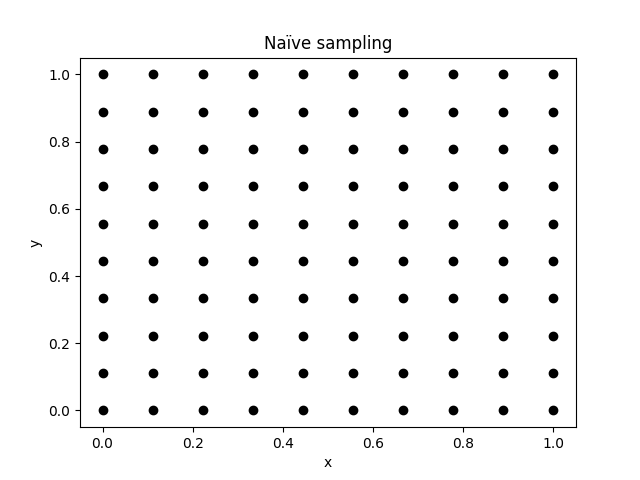
\includegraphics[width=\textwidth]{sampling-naive.png}
        \caption{Naïve strategy}
        \label{fig:sampling-naive}
    \end{subfigure}
    \hfill
    \begin{subfigure}[b]{0.49\textwidth}
        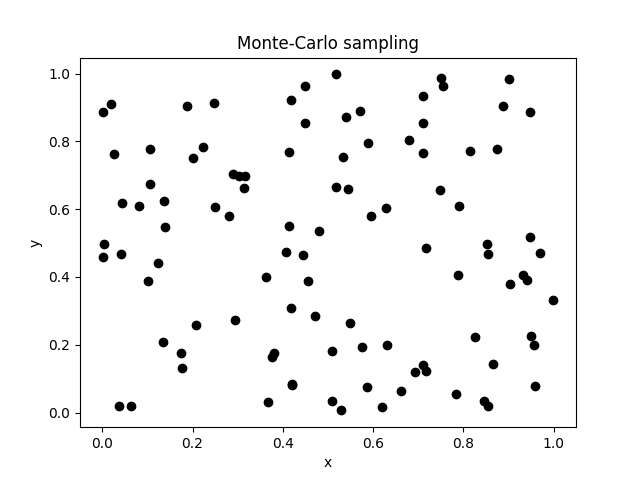
\includegraphics[width=\textwidth]{resources/images/sampling-monte-carlo.png}
        \caption{Monte-Carlo strategy}
        \label{fig:sampling-monte-carlo}
    \end{subfigure}
    \caption{Basic sampling strategies}
\end{figure}

\begin{figure}[h!]
    \centering
    \begin{subfigure}[b]{0.49\textwidth}
        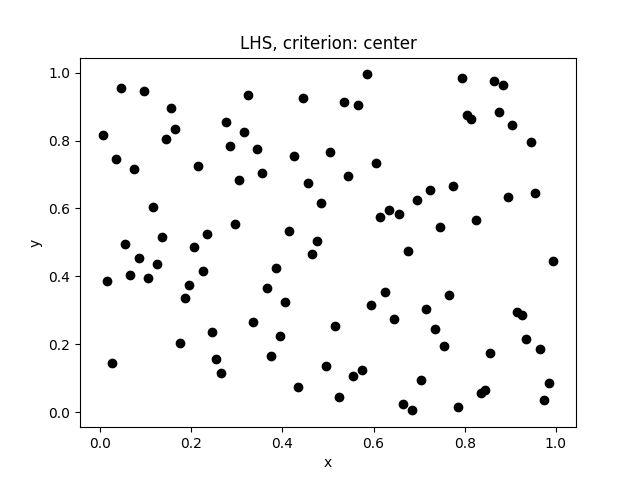
\includegraphics[width=\textwidth]{resources/images/sampling-lhs-center.png}
        \caption{LHS with center criterion}
        \label{fig:sampling-lhs-center}
    \end{subfigure} 
    \hfill
    \begin{subfigure}[b]{0.49\textwidth}
        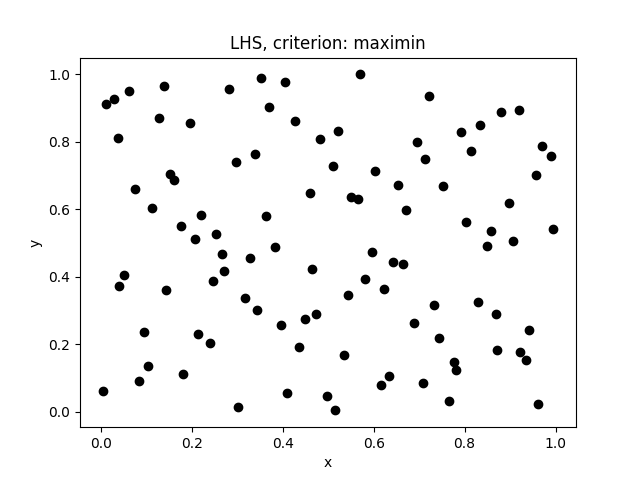
\includegraphics[width=\textwidth]{resources/images/sampling-lhs-maximin.png}
        \caption{LHS with max min distance criterion}
        \label{fig:sampling-lhs-maximin}
    \end{subfigure} 
    \hfill
    \begin{subfigure}[b]{0.49\textwidth}
        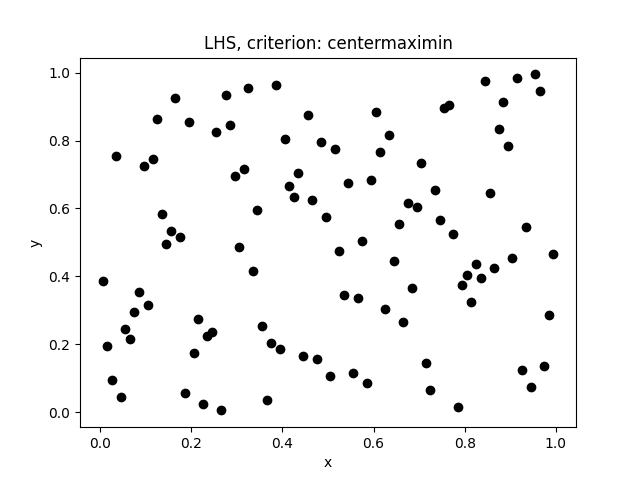
\includegraphics[width=\textwidth]{resources/images/sampling-lhs-centermaximin.png}
        \caption{LHS with max min distance and center criterion}
        \label{fig:sampling-lhs-centermaximin}
    \end{subfigure} 
    \hfill
    \begin{subfigure}[b]{0.49\textwidth}
        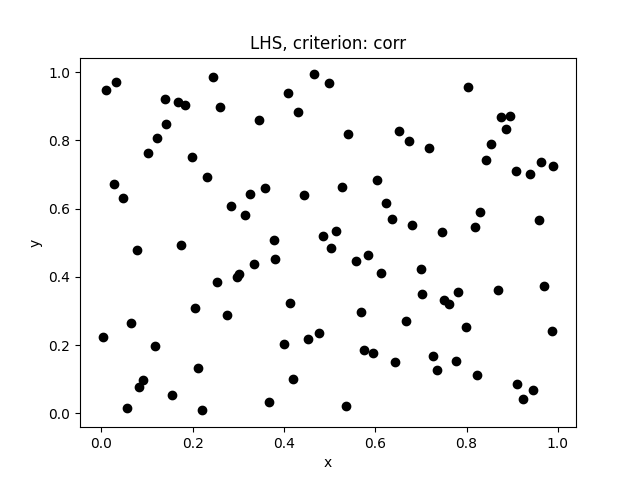
\includegraphics[width=\textwidth]{resources/images/sampling-lhs-corr.png}
        \caption{LHS with correlation criterion}
        \label{fig:sampling-lhs-corr}
    \end{subfigure} 
    \caption{Latin hypercube sampling strategies with every criterion}
\end{figure}

From these 2-dimensional illustration it is clear that the latin hypercube sampling performs best, the naive sampling featuring too much regularities that is not wanted, as they may introduce some bias, and Monte-Carlo sampling tends to make more clusters of samples, that would be inefficient (indeed, making two times the same simulation is useless).

\subsection{Generation of the dataset}

With the input samples now obtained, the next step is now to compute the simulations on each of these points.

But this task is not trivial: we don't have the data that corresponds to these exact configuration. It is thus needed to craft some new simulation settings given a reference, that is the year 2019.

\subsubsection{Adjusting function}
To do so, Dispa-SET disposes of utility functions that do just that, adjusting the capacities, i.e., the power ouputs of the units, in function of some parameters.

These adjusting functions have been specifically developped for this topic by Vidal in her master thesis \cite{carlas-thesis}.

\begin{itemize}
    \item \texttt{adjust\_flexibility} modifies installed capacities to reach the desired $Share_{flex}$.
    
    To do so, it first computes the target capacity, by multiplying the total capacity by the desired $Share_{flex}$. It then add or subtracts the missing or exceeding flexible unit power capacity to each zone, weighting by their total capacity, following Equation \ref{equation:flex-cap-weight}.

    \begin{equation}
        capacity_{z,new} = capacity{z,old} + \frac{capacity_{z,new}}{\sum_x capacity_{x,old}} (target-actual)
        \label{equation:flex-cap-weight}
    \end{equation}

    \item \texttt{adjust\_capacity} applies a linear scaling to the power output of some given set of units, in particular, it will be called multiples times to adjust the storage, PV and wind capacities.
    
    Scaling factors applied are summarized in Table \ref{table:scaling-factors}.

    \begin{table}[h]
        \centering
        \begin{tabular}{|l l|}
            \hline  
            Units              & Scaling factor    \\ \hline
            $Storage_{units}$  & $Share_{storage}$ \\ 
            $Wind_{units}$     & $\frac{CapacityRatio \cdot Share_{wind}}{AF_{wton}}$ \\
            $PV_{units}$       & $\frac{CapacityRatio \cdot Share_{PV}}{AF_{PV}}$ \\ \hline
        \end{tabular}
        \caption{Scaling factors applied to different units}
        \label{table:scaling-factors}
    \end{table}

    \item \texttt{adjust\_rntc} applies a linear scaling to each zonal NTC time series.
\end{itemize}

\subsubsection{Extracted outputs}

As every simulation runs outputs a lot more than only the curtailment and lost load values, some other outputs variables will be extracted from the simulations, while not directly useful for the time being.

Of course, these may reveal themselves useful for future work.

All the outputs extracted from the simulations are displayed in Table \ref{table:values-extracted}.

\begin{table}[h]
    \centering
    \begin{tabular}{|l c|l c|}
		\hline
		Parameter & Unit & Parameter & Unit \\
		\hline
		Cost            & €/MWh & Shedding & TWh \\
		Congestion      & h     & LostLoad & TWh \\
		PeakLoad        & MW    & CF gas  & [$\cdot$] \\
		MaxCurtailment  & MW    & CF nuc  & [$\cdot$] \\
		MaxLoadShedding & MW    & CF wat   & [$\cdot$] \\
		Demand          & TWh   & CF win   & [$\cdot$] \\
		NetImports      & TWh   & CF sun   & [$\cdot$] \\
		Curtailment     & TWh   &  &  \\
		\hline
	\end{tabular}
	\caption{Values extracted from each simulations}
	\label{table:values-extracted}
\end{table}

\subsection{Implementation}

One simple, yet important notice: running all of these simulation is not feasible on a basic hardware. This arises the need for the cluster use, and thus of submitting these as jobs on the cluster.

As the NIC5 cluster provided by CÉCI is obviously shared, one needs to manage the submitted jobs appropriately. In our case, we simply have the same program to be run a bunch of times, that are jobs independent of each other.

\subsubsection{Steps}
For a complete experiment to be completed, these steps have to be followed:
\begin{enumerate}
    \item Generating the reference simulation, to extract the data that will be manipulated by the adjusting function
    \item For each sample, do:
    \begin{enumerate}
        \item Call the adjusting function and create the simulation directory, with all the simulation input data
        \item Call GAMS in this simulation directory
        \item Fetch GAMS outputs in this directory
    \end{enumerate}
\end{enumerate}

\subsubsection{Scripts and code}

The steps presented above almost map to a script or function written. The flow of the dataset generation is as described here.

\begin{enumerate}
    \item The SLURM script \texttt{main.sh} is submitted on the cluster. It fetches relevant data in the \texttt{config.py} script.
    \item It submits the generation of the reference simulation as another job on the cluster and waits for its completion.
    \item It calls \texttt{sampling.py} with argument \texttt{--sample-only}, that will create the \texttt{samples.csv} file containing all the samples.
    \item It prepares the file \texttt{dataset.csv} by writing its header line.
    \item It finally runs the bash script \texttt{launch-job-series.sh}, that will submit some fixed number of sample jobs, as an array, through the SLURM script \texttt{launch-simulation-jobs.sh}.
    \item Each sample job runs:
    \begin{enumerate}
        \item The simulation directory is prepared by calling the \texttt{sampling.py} script with argument \texttt{--prepare-one} and the index of this simulation (it reads the corresponding line in \texttt{samples.csv}).
        \item GAMS is called on the simulation directory.
        \item The simulation results are read with \texttt{read\_results.py --single}, then outputted to \texttt{dataset.csv}.
        \item The simulation directory is cleaned.
    \end{enumerate}
\end{enumerate}

\subsubsection{Technical aspects}

During the creation of this set of scripts, some technical details require specific attention:
\begin{itemize}
    \item The GAMS solver spawns threads for efficiency, the number of threads must not exceed the number of CPUs allocated by SLURM for that job, otherwise it will disturb the whole node on which it is running, including unrelated jobs.
    \item The total amount of each prepared simulation directory is too large to fit on the allocated disk memory on the cluster.
    \item The Dispa-SET ajdusting function do not write adjusted data to a directory if this directory already exists before the function is called
\end{itemize}

\mywarning{Should I write more about the "history" of the scripts ?}

\subsubsection{Dataset fields}

For completeness, all the fields in the created dataset in \texttt{dataset.csv} are shown on Table \ref{table:dataset-fields}.

\begin{table}[h]
    \centering
	\begin{tabular}{|l c|l c|}
		\hline
		Parameter & Unit & Parameter & Unit \\
		\hline
		Cost            & €/MWh & CF nuc        & [$\cdot$] \\
		Congestion      & h    & CF wat         & [$\cdot$] \\
		PeakLoad        & MW   & CF win         & [$\cdot$] \\
		MaxCurtailment  & MW   & CF sun         & [$\cdot$] \\
		MaxLoadShedding & MW   & Capacity ratio & [$\cdot$] \\
		Demand          & TWh  & Share flex     & [$\cdot$] \\
		NetImports      & TWh  & Share sto      & [$\cdot$] \\
		Curtailment     & TWh  & Share Wind     & [$\cdot$] \\
		ENS             & TWh  & Share PV       & [$\cdot$] \\
		CF gas          & \%   & rNTC           & [$\cdot$] \\
		\hline
	\end{tabular}
	\caption{Dataset fields}
	\label{table:dataset-fields} 
\end{table}
\section{Surrogate model training}

\subsection{Overview}

This section presents the training process that lead to the description and definition of the target surrogate model, given a ready to use dataset, and the desired characteristics.

This is a straightforward example of a regression problems, that is to predict some output features from the input features, given a number of training example, that is the dataset. This is a typical machine learning problem, and will be tackled as such.

\subsection{Machine learning methods}

In the following, some machine learning algorithms for regression problems \cite{machine-learning-class} are assessed.

\subsubsection{K nearest neighbors}

In this setting, the K-nearest neighbors (k-NN) methods would be one of the easiest to implement\footnote{Using for example \href{https://scikit-learn.org/stable/modules/neighbors.html\#nearest-neighbors-regression}{scikit-learn}\cite{scikit-learn} module in python}. Indeed, these simply require a single parameter value $k$ and output the average value of the output features of the $k$ nearest neighbors, computing a distance on the input features.

This will come with the drawback of not being able to learn quick variations in the outputs. What is considered too problematic, as these critical points would need to be properly modelled for the reliability of the surrogate model.

\subsubsection{Decision trees}

Decision trees, and extremely randomized trees \cite{extremely-randomized-trees} another category of easy to implement\footnote{Again, using \href{https://scikit-learn.org/stable/modules/ensemble.html\#forests-of-randomized-trees}{scikit-learn}} machine learning methods, as they also come with a limited, fixed number design parameters.

But these also come with the drawback of having a piecewise constant output, and as stated above, it is required to be able to represent significantly fast variations in the output. Although it is possible to mimic with many successive steps, being peicewise constant will now introduce non linearities in the outputs, that is, unwanted steps in the prediction.

\subsubsection{Kernel-based methods\label{section:kernel-methods}}

One may consider to apply a kernel method with one of the other method mentioned above. While this may indeed improve the quality of the resulting model, and also solve the issue that was representing fast changes in the output, there is a main, almost trivial issue with them. Obviously, one need a kernel, but what kernel?

As there are no ready-to-use kernel for this specific case, and that finding such a kernel would be a hard task, kernel methods are abandonned.

\subsubsection{Artificial neural network}

Artificial neural networks (ANN) are used in this work to build our surrogate model. These kind of methods provide a large flexibility, due to their entirely customizable architecture, as well as a large learning capacity. This makes them able to modelize with good accuracy some complex, non-linear functions.

In most recent applications of these ANNs, a lot of different strategies are used to process the data efficiently. For example, convolutional layers convey a lot of meaning in the context of image processing, or transformers are well suited to process sequences\cite{deep-learning-class}.

In this case, the inputs boils down to the 6 variables values, listed in Table {table:reference-values}. There are no patterns in this data, because even if their actual values were correlated in some way, the simulations dataset we have as an input at this stages has its input features drawn from a latin hypercube sampling, meaning they have a fixed, very low correlation. This correlation originates from the fact that the sampling aims at optimizing the design space coverage, not from a meaningful, exploitable source.

Thus, a simple multi-layer perceptron (MLP) architecture is chosen, and the next requirement is to describe the characteristics of that MLP, that are:
\begin{itemize}
    \item The number of layers
    \item The numbers of neurons in each layers
    \item The activation function at each layer
\end{itemize}
\section{The surrogate model}

\subsection{Overview}

This section presents the training process that have led to the description and definition of the target surrogate model, given a ready to use dataset, and the desired characteristics.

This is a straightforward example of a regression problems, aiming to predict some output features from the input features, given a number of training example in a dataset. This is a typical machine learning problem, and is be addressed accordingly.

Initially, the performance of different methods are measured and the best one is selected. Then, a model is trained and evaluated, forming the core surrogate model.

\subsection{Machine learning methods}

This subsection assesses some of the most common machine learning algorithms for regression problems \cite{machine-learning-class}.

\subsubsection{K nearest neighbors}

In this context, the K-nearest neighbors (k-NN) methods is among one of the easiest to implement, using tools like the \href{https://scikit-learn.org/stable/modules/neighbors.html\#nearest-neighbors-regression}{scikit-learn} \cite{scikit-learn} module in python. Indeed, these simply require a single parameter value $k$ and output the average value of the output features of the $k$ nearest neighbors, computing a distance on the input features.

This will come with the drawback of not being able to learn quick variations in the outputs, as the averaging over the nearest sample points will filter out high frequency variations.

Results obtained with k-NN for various values of $k$ are shown in Table \ref{tab:results-knn}.

\begin{table}[h]
    \centering
    \begin{tabular}{|l|l|}
        \hline
        k & Validation error \\ \hline
        4  & 0.05082837 \\
        5  & 0.051765025 \\
        6  & 0.047083396 \\
        7  & 0.046183977 \\
        8  & 0.049501333 \\
        9  & 0.049218103 \\
        10 & 0.04949624 \\
        11 & 0.05036374 \\
        12 & 0.050881956 \\
        13 & 0.05243453 \\
        14 & 0.052941263 \\
        15 & 0.05362743 \\
        16 & 0.05440363 \\ \hline
    \end{tabular}
    \caption{Results obtained with k-NN}
    \label{tab:results-knn}
\end{table}

The best performance is obtained for $k$ equal to 7. Smaller values increase the error due to overfitting, while larger values suffer from underfitting, resulting in larger errors.

\subsubsection{Decision trees}

Decision trees, along with extremely randomized trees \cite{extremely-randomized-trees} are easy to implement\footnote{Again, using \href{https://scikit-learn.org/stable/modules/ensemble.html\#forests-of-randomized-trees}{scikit-learn}} machine learning methods as well, as they also involve a constrained and fixed number design parameters.

These methods, however, exhibit the limitation of producing piecewise constant output, and as stated above, it is required to be able to represent significantly fast variations in the output. Although it is possible to mimic using many successive steps, being peicewise constant will now introduce non linearities in the outputs, that is, unwanted steps in the prediction.

Results obtained with decision trees are shown in Table \ref{tab:trees-results}.

\begin{table}[h]
    \centering
    \begin{tabular}{|c|c|}
        \hline
        Number of trees & Validation error \\ \hline
        25  & 0.02385 \\
        35  & 0.02347 \\
        45  & 0.02275 \\
        55  & 0.02342 \\
        65  & 0.02361 \\
        75  & 0.02272 \\
        85  & 0.02360 \\
        95  & 0.02255 \\
        105 & 0.02294 \\
        115 & 0.02379 \\
        125 & 0.02263 \\
        135 & 0.02232 \\
        145 & 0.02317 \\ \hline
    \end{tabular}
    \caption{Results obtained with random forests}
    \label{tab:trees-results}
\end{table}

The highest accuracy is achieved with 135 trees. However in this case, the results are not as straightforward as for the k-NN technique, that showed a monotonic decrease, the minimum then an increase. As randomness is involved when choosing the splits when building the trees, the results are subject to a slight variance, inducing less obvious results. However, after 145 trees, the error starts steadily increasing.

These performance are better than the nearest neighbors method, but do not perform as good as the following techniques.

\subsubsection{XGBoost}

XGBoost is currently one of the most popular machine learning technique \cite{XGBoost}. It actually is an efficient implementation of a machine learning method, tree boosting.

Boosting aims to construct a string predictive model from so-called weak learners, which in this case, are trees. Each learner is trained on the error of the output of the previous model, so that the previous output plus the newly trained learner output is a better prediction of the target output. Moreover, the samples are weighted in favor of the ones that were badly predicted by the previous model, in order to make sure we correct past mistakes.

In tree boosting, the main hyper-parameters are:
\begin{itemize}
    \item the number $n$ of weak learners stacked
    \item the \textit{learning rate}, a constant factor applied to the target difference (target output minus previous model output)
    \item the maximum depth of the weak learners
\end{itemize}

Resulting performance for some values of the hyper-parameters are reported in Table \ref{tab:results-xgboost}.

XGBoost's results are really good, achieving at best around 0.006 mean squared error on the validation set. This is not surprising given that this technique is quite popular in the literature. 

It is important to note that the method was tested over a previous version of the dataset (the one produced in \cite{carlas-thesis}) and not on the one generated in this thesis because the results were not yet available. The performance metrics should however not very dramatically between the former and the latter version of the dataset.
% Actually, for the first testing stage where the dataset created in this work was not available, the dataset from C. Vidal's work has been used as a first test. In this context, the results obtained with XGBoost outperformed the best neural network architecture.

\begin{table}[h!]
    \centering
    \begin{tabular}{|l|l|l|l||l|l|l|l||l|l|l|l|}
        \hline
        d & lr   & n    & err      & d  & lr   & n    & err      & d & lr   & n    & err      \\ \hline
        3 & 0.03 & 10   & 0.5248   &  4 & 0.1  & 10   & 0.1564   & 5 & 0.2  & 10   & 0.03299  \\
        3 & 0.03 & 20   & 0.3367   &  4 & 0.1  & 20   & 0.04522  & 5 & 0.2  & 20   & 0.01088  \\
        3 & 0.03 & 50   & 0.1100   &  4 & 0.1  & 50   & 0.01059  & 5 & 0.2  & 50   & 0.007287 \\
        3 & 0.03 & 100  & 0.033627 &  4 & 0.1  & 100  & 0.007168 & 5 & 0.2  & 100  & 0.006907 \\
        3 & 0.03 & 200  & 0.01294  &  4 & 0.1  & 200  & 0.006018 & 5 & 0.2  & 200  & 0.006681 \\
        3 & 0.03 & 500  & 0.007804 &  4 & 0.1  & 500  & 0.005489 & 5 & 0.2  & 500  & 0.006624 \\
        3 & 0.03 & 1000 & 0.006434 &  4 & 0.1  & 1000 & 0.005325 & 5 & 0.2  & 1000 & 0.006623 \\
        3 & 0.03 & 2000 & 0.005553 &  4 & 0.1  & 2000 & 0.005294 & 5 & 0.2  & 2000 & 0.006623 \\
        3 & 0.1  & 10   & 0.1886   &  4 & 0.2  & 10   & 0.04046  & 6 & 0.03 & 10   & 0.4870   \\
        3 & 0.1  & 20   & 0.06469  &  4 & 0.2  & 20   & 0.01313  & 6 & 0.03 & 20   & 0.2861   \\
        3 & 0.1  & 50   & 0.01586  &  4 & 0.2  & 50   & 0.007588 & 6 & 0.03 & 50   & 0.06760  \\
        3 & 0.1  & 100  & 0.009350 &  4 & 0.2  & 100  & 0.006579 & 6 & 0.03 & 100  & 0.01544  \\
        3 & 0.1  & 200  & 0.007291 &  4 & 0.2  & 200  & 0.006219 & 6 & 0.03 & 200  & 0.007516 \\
        3 & 0.1  & 500  & 0.005978 &  4 & 0.2  & 500  & 0.006029 & 6 & 0.03 & 500  & 0.006548 \\
        3 & 0.1  & 1000 & 0.005558 &  4 & 0.2  & 1000 & 0.006007 & 6 & 0.03 & 1000 & 0.006381 \\
        3 & 0.1  & 2000 & 0.005375 &  4 & 0.2  & 2000 & 0.006007 & 6 & 0.03 & 2000 & 0.006343 \\
        3 & 0.2  & 10   & 0.059425 &  5 & 0.03 & 10   & 0.4916   & 6 & 0.1  & 10   & 0.1368   \\
        3 & 0.2  & 20   & 0.02037  &  5 & 0.03 & 20   & 0.2894   & 6 & 0.1  & 20   & 0.03335  \\
        3 & 0.2  & 50   & 0.009474 &  5 & 0.03 & 50   & 0.07119  & 6 & 0.1  & 50   & 0.008382 \\
        3 & 0.2  & 100  & 0.007554 &  5 & 0.03 & 100  & 0.01647  & 6 & 0.1  & 100  & 0.006850 \\
        3 & 0.2  & 200  & 0.006287 &  5 & 0.03 & 200  & 0.006834 & 6 & 0.1  & 200  & 0.006594 \\
        3 & 0.2  & 500  & 0.005976 &  5 & 0.03 & 500  & 0.005326 & 6 & 0.1  & 500  & 0.006504 \\
        3 & 0.2  & 1000 & 0.005935 &  5 & 0.03 & 1000 & 0.005069 & 6 & 0.1  & 1000 & 0.006491 \\
        3 & 0.2  & 2000 & 0.005894 &  5 & 0.03 & 2000 & 0.004952 & 6 & 0.1  & 2000 & 0.006491 \\
        4 & 0.03 & 10   & 0.5013   &  5 & 0.1  & 10   & 0.1425   & 6 & 0.2  & 10   & 0.0302   \\
        4 & 0.03 & 20   & 0.3042   &  5 & 0.1  & 20   & 0.03577  & 6 & 0.2  & 20   & 0.01046  \\
        4 & 0.03 & 50   & 0.08414  &  5 & 0.1  & 50   & 0.008340 & 6 & 0.2  & 50   & 0.007929 \\
        4 & 0.03 & 100  & 0.02168  &  5 & 0.1  & 100  & 0.006145 & 6 & 0.2  & 100  & 0.007743 \\
        4 & 0.03 & 200  & 0.008364 &  5 & 0.1  & 200  & 0.005640 & 6 & 0.2  & 200  & 0.007651 \\
        4 & 0.03 & 500  & 0.005841 &  5 & 0.1  & 500  & 0.005433 & 6 & 0.2  & 500  & 0.007622 \\
        4 & 0.03 & 1000 & 0.005203 &  5 & 0.1  & 1000 & 0.005371 & 6 & 0.2  & 1000 & 0.007622 \\
        4 & 0.03 & 2000 & 0.004922 &  5 & 0.1  & 2000 & 0.005371 & 6 & 0.2  & 2000 & 0.007622 \\ \hline
    \end{tabular}
    \caption{Results for some values of the XGBoost parameters. The learning rate is labelled "lr", the maximum depth "d" and the number of estimators n, while the validation error is denoted by "err".}
    \label{tab:results-xgboost}
\end{table}

The best performance is observed with a maximum depth of 4, a learning rate set to 0.03 and 2000 trees. Further fine-tuning may slightly improve this value, in particular reduce the learning rate and increase the number of trees even more, but further investigation showed that the performance stagnate starting from 1800.

% As there are tree dimensions to take into account, we need to find combination of values. Results in Table \ref{tab:results-xgboost} indicate that there is a balance to find between the depth of the approximators and their number. Sh

\subsubsection{Kernel-based methods\label{section:kernel-methods}}

One might consider applying a kernel method with one of the other method mentioned above. While this may indeed improve the quality of the resulting model, and also solve the issue that was representing fast changes in the output, nevertheless, finding a suitable kernel is a difficult.

Since there is no ready-to-use kernel for this specific case, and that finding such a kernel would be a hard task, kernel methods are discarded.

\subsubsection{Artificial neural network}

Artificial neural networks (ANN) are used in this work to build our surrogate model. These types of methods offer a large flexibility, due to their entirely customizable architecture, as well as a large learning capacity. This makes them able to modelize with good accuracy some complex, non-linear functions.

In most recent applications of these ANNs, a lot of different strategies are used to process the data efficiently. For example, convolutional layers convey a lot of meaning in the context of image processing, or transformers are well suited to process sequences \cite{deep-learning-class}.

In this case, the inputs boils down to the 6 variables values, listed in Table \ref{table:reference-values}. There are no patterns in this data, because even if their actual values were correlated in some way, the simulations dataset we have as an input at this stages has its input features drawn from a latin hypercube sampling, meaning they have a fixed, very low correlation. This correlation originates from the fact that the sampling aims at optimizing the design space coverage, not from a meaningful, exploitable source.

Thus, a simple multi-layer perceptron (MLP) architecture is chosen, and the next requirement is to describe the characteristics of that MLP, that are:
\begin{itemize}
    \item The number of layers
    \item The numbers of neurons in each layers
    \item The activation function at each layer
\end{itemize}

Some experiments are run to provide some baselines for getting a first approximation of what performs well. These results are presented in Table \ref{tab:nn-results}.

\begin{table}[h!]
    \centering
    \begin{tabular}{|p{0.7\textwidth}|p{0.2\textwidth}|}
        \hline
        Architecture & Validation error \\ \hline
        (180, 'relu', 0.4), (100, 'tanh', 0.4) & 0.00484 \\
        (180, 'relu', 0.4), (100, 'tanh', 0.4) & 0.00499 \\
        (180, 'relu', 0.4), (100, 'tanh', 0.4) & 0.00480 \\
        (70, 'relu', 0.5), (70, 'relu', 0.5) & 0.04538 \\
        (100, 'relu', 0.4), (100, 'relu', 0.4) & 0.02506 \\
        (100, 'relu', 0.5), (100, 'relu', 0.5) & 0.04111 \\
        (100, 'relu', 0.6), (100, 'relu', 0.6) & 0.04481 \\
        (100, 'relu', 0.7), (100, 'relu', 0.7) & 0.10410 \\
        (80, 'relu', 0.7), (80, 'relu', 0.7) & 0.06514 \\
        (150, 'relu', 0.6), (100, 'relu', 0.6) & 0.02693 \\
        (250, 'relu', 0.4), (125, 'relu', 0.4) & 0.01295 \\
        (200, 'relu', 0.5), (125, 'relu', 0.5) & 0.01734 \\
        (200, 'relu', 0.5), (125, 'tanh', 0.5) & 0.00532 \\
        (200, 'relu', 0.4), (125, 'tanh', 0.4) & 0.00555 \\
        (200, 'relu', 0.4), (100, 'tanh', 0.4) & 0.00581 \\
        (150, 'relu', 0.45), (100, 'tanh', 0.45) & 0.00585 \\
        (150, 'relu', 0.5), (100, 'tanh', 0.5) & 0.00603 \\
        (150, 'relu', 0.4), (80, 'tanh', 0.4) & 0.00597 \\
        (220, 'relu', 0.5), (125, 'relu', 0.5) & 0.01086 \\
        (250, 'relu', 0.5), (125, 'relu', 0.5) & 0.02421 \\
        (250, 'tanh', 0.4), (125, 'tanh', 0.4) & 0.04193 \\
        (200, 'relu', 0.5), (150, 'relu', 0.5), (100, 'relu', 0.4) & 0.07372 \\
        (120, 'relu', 0.4), (120, 'relu', 0.4), (120, 'relu', 0.4) (120, 'relu', 0.4), (80, 'relu', 0.4) & 0.12163 \\
        (50, 'relu', 0.3), (50, 'relu', 0.3), (50, 'relu', 0.3), (50, 'relu', 0.3) & 0.08267 \\
        (50, 'relu', 0.4), (50, 'relu', 0.4), (50, 'relu', 0.4), (50, 'relu', 0.4) & 0.14292 \\
        (50, 'relu', 0.2), (50, 'relu', 0.2), (50, 'relu', 0.2) & 0.02622 \\
        (50, 'relu', 0.2), (50, 'relu', 0.2), (50, 'relu', 0.2), (50, 'relu', 0.2) & 0.05221 \\
        (50, 'relu', 0.3), (50, 'relu', 0.3), (50, 'relu', 0.3) & 0.05723 \\
        (50, 'relu', 0.4), (50, 'relu', 0.4), (50, 'relu', 0.4) & 0.08706 \\
        (150, 'relu', 0.5), (150, 'relu', 0.5), (150, 'relu', 0.5) & 0.07769 \\
        (150, 'relu', 0.5), (100, 'relu', 0.5), (100, 'relu', 0.5) & 0.08809 \\
        (150, 'relu', 0.5), (150, 'relu', 0.5), (100, 'relu', 0.5) & 0.08098 \\
        (200, 'relu', 0.5), (200, 'relu', 0.5), (150, 'relu', 0.5) & 0.07682 \\
        (190, 'relu', 0.5), (190, 'relu', 0.5), (140, 'relu', 0.5) & 0.06489 \\
        (200, 'relu', 0.5), (200, 'relu', 0.5), (150, 'relu', 0.5), (30, 'relu', 0.3) & 0.08749 \\
        (200, 'relu', 0.5), (200, 'relu', 0.5), (150, 'relu', 0.5), (50, 'relu', 0.3) & 0.09094 \\
        (200, 'relu', 0.5), (200, 'relu', 0.5), (200, 'relu', 0.5) & 0.07010 \\
        (150, 'relu', 0.5), (150, 'relu', 0.5), (150, 'relu', 0.5), (150, 'relu', 0.5) & 0.13490 \\ \hline
    \end{tabular}
    \caption{Results for some architectures of neural networks. Architectures are formatted as a list of layers, which are written as ($n$, $a$, $p$) tuples, where $n$ is the number of neurons, $p$ the dropout value and $a$ the activation function}
    \label{tab:nn-results}
\end{table}

These result outperform every other method. The fact that different but close architecture show similar performance brings some confidence about the reproducibility: the random initialization of the weights in the network could have led to an exceptionally good model. Moreover, several runs of the same architecture yield similar ouputs, validating this intuition.

It is worth mentioning that some larger network architecture, \textit{e.g.} $(300, 'relu', 0), (300, 'relu', 0),$ $(200, 'relu', 0)$ achieved really good results, even slightly better than the best one. However these were not implementing dropout, so that they are high changes of being subject to overfitting. If dropout is added, the observed performance decrease, confirming the overfitting hypothesis.

This is why the relative smallness of the network is a strength, as it will also act against overfitting, as having fewer parameters leaves less room for learning noise.

\subsubsection{Selection of the machine learning technique and parametrization}

In the end, neural networks are opted for. They benefit from the best performance in terms of mean squared error on the validation test, but neural networks MLPs also present the following advantages:
\begin{itemize}
    \item They are relatively lightweight, in comparison to the K-nearest neighbors methods, that needs to store the entire dataset, and the randomized trees, that need to store its trees structures. Neural networks only needs their weights that are fairly small with this few input variables.
    \item Grasp non-linear behaviour with accuracy
\end{itemize}

Preliminary experiments basically consist in the test undertaken to assess the performance of different architectures (reported in Table \ref{tab:nn-results}). While the firsts steps of testing used another dataset that available at the time, ultimately the generated dataset was the only one in use for this assessments.

The architecture is selected as the optimal one among baselines, and is provided in Table \ref{tab:nn-layers}. While hyper-parameter tuning may have produced another result, the latter could potentially suffer from overfitting, as described above. 

\begin{table}[h!]
    \centering
    \begin{tabular}{|l|l|l|}
        \hline
        Layer index & Layer type & Weights count \\ \hline
        1 & Fully connected linear layer, 6 inputs to 180 outputs & $6\times 180 = 1080$ \\
        2 & ReLU activation function & 0 \\
        3 & Dropout layer, with $p=0.4$ & 0 \\
        4 & Fully connected linear layer, 180 inputs to 100 inputs & $180\times 100=18000$ \\
        5 & $\tanh$ activation function & 0 \\
        6 & Dropout layer, with $p=0.4$ & 0\\
        7 & Fully connected linear layer, 100 inputs to 2 outputs & $100\times 2$ \\ \hline
    \end{tabular}
    \caption{Description of the layers of in the selected architecture for the model}
    \label{tab:nn-layers}
\end{table}

Consequently, the final parameterization of the model involves the setting of all its weights, that lie in layers 1, 4 and 7. The total count of parameters adds up: $1080 + 18000 + 200 = 19280$.

\subsection{Machine learning aspects}

\subsubsection{Validation and testing\label{ssec:val-testing}}

In machine learning, validation and testing are crucial steps in order to ensure the performance of a model. To implement these, one must separate the data into three sets.

\begin{itemize}
    \item The validation set is used for hyperparameters tuning. Given its influence on the model, it can introduce bias into the model.
    \item The test set is used to evaluate the model's performance, on unseen data.
    \item The training set is used to train the model.
\end{itemize}

% Typically, the data is split into three subsets. However, in this setting, the training, input data comes from a latin hypercube, and can be generated. Taking this into account, one may then consider the use of different LHS.
Typical machine learning applications dispose of a single, fixed dataset, that has to be split to constitute three desired sets. However, in this context, we can easily run sets of simulations to obtain more data points, from another LHS. It is interesting to consider generating more than a single dataset from a unique LHS.

For the training set, joining different sets drawn with LHS is not expected to improve performance. As the LHS are independent of each other, there is a great chance to draw samples that are really close to each other, or worse, equal, what the LHS aims to avoid.

On the other hand, using a set drawn from a different LHS (than the one used for the training set) for testing and validation is interesting. This will provide data that spans the whole input space, but not yet exactly the same as the data used for training. Thanks to the input space coverage, the evaluation made at testing will be more extensive, and thanks to being independent of the training data, this evaluation should remain unbiased. 

Conversely, the validation set being sampled from a LHS now providing a guarantee that it spans the whole space could make the work of the learning agent easier, giving it access to each of the LHS sample from the training set.

However promising, this approach will not be done in this work, to ensure that the unbiased property of the trained model persists, and that the term "validation error" keeps the exact same meaning as in the literature.

\subsubsection{Overfitting}

An inherent challenge to machine learning methods is the overfitting, or its opposite, underfitting. These terms refer to the cases where the training is respectively too specific to the training data, and not enough specific.

Overfitting is a result of excessive learning, leading to learning some noise or some particularities of the dataset, while underfitting means that there is not enough learning, so that the model is not able to represent all the cases, even the one that are well represented in the available data.

The main tool used to prevent it in a neural network is the dropout. During the training phases, each neuron on a layer will have some probability $p$, typically between 0.3 and 0.5, of being set to 0, independently of its value. This methods ensures that the network will not be excessively relying on some neurons in its output. During testing oviously, the dropout is removed and all neurons are functional.

\subsubsection{Underfitting}

On the other hand, underfitting means there is not enough learning happening. For example, a neural network with only 2 neurons corresponding to the ouputs could not learn any non-linear functions, with some tweaks due to the eventual activation function.

In this setting, although underfitting is still a shortfall, it is not regarded as bad as the overfitting. The latter introduces errors that come from noise that is completely random, inevitably introducing imprecisions. But we keep in mind that the target to be approximated, that are outputs from the Dispa-SET model, are themselves an approximation, though accurate, of the reality. So if these are subject to some bias or imperfections, the best model would learn them as well.

Because an underfitting model of the dataset created using Dispa-SET would still be a decent estimate of the reality, which is the primary objective in this context, underfitting is preferable to overfitting.

These will have to be assessed during training to ensure the validity of the model.

\subsubsection{Bias\label{ssec:bias}}

An other source of imprecision in machine learning is the bias. This relates to the fact that there exist some noise in the data, that cannot be filtered out, or imprecisions in the assumptions, that inevitably conducts to noise in the output.

However, in this setting, there is very little one could implement to reduce its significance. First, the data points have been drawn from a latin-hypercube sampling strategy, that precisely aims at spreading the samples equitably all over the input space. Then, the output features were computed from a Dispa-SET run on this sample.

Hence, the primary source of bias that can be addressed pertains to model training inaccuracies resulting from suboptimal model design.

The other plausible source of bias is the simulation made in Dispa-SET. Of course, Dispa-SET is also itself a model, thus relying on some assumptions and subject to its own modelling of the reality. And as such, it may introduce a bias in its computations, that will necessarily be learned by the surrogate model. But there is no way to assess this bias, and obviouly Dispa-SET itself focuses on making that bias as negligible as possible.

This consideration is of interest, as Dispa-SET has multiple formulations, namely LP and MILP, that then have different bias with respect to reality.

\subsection{Training}

\subsubsection{Implementation}

All the files for this section lie in the \texttt{nn} folder.

The implementation of the training process comprises the following files:
\begin{itemize}
    \item \texttt{config.py}, that holds all the high-level specifications of the training, such as the names of the outputs, the train-test-validation set ratios, the number of epochs etc.
    \item \texttt{model.py}, that contains the function building the model, thus the definition of the neural network's architecture.
    \item \texttt{baselines.py}, that contains code to train models with pre-defined architectures, in order to quickly and easyly have an overview of the order of magnitude involved.
    \item \texttt{train.py}, that contains the code for the hyperparameter tuning and model training.
    \item \texttt{view.py}, that contains the utilities to visualize the results.
    \item \texttt{tests.py}, that contains the testing of the other machine learning methods (k-NN, trees, XGBoost)
    \item \texttt{data}, \texttt{logs}, \texttt{models} directories, that contain the datasets, the runs' logs, and the trained models respectively.
\end{itemize}

\subsubsection{Results}

The chosen architecture is a two-layer network:
\begin{enumerate}
    \item 180 neurons, ReLU activation, 0.4 chance of dropout
    \item 100 neurons, hyperbolic tangent activation, 0.4 chance of dropout
\end{enumerate}

The mean squared error over the training epochs is shown in Figure \ref{fig:nn-validation-error-curve}.

\begin{figure}[h]
    \centering
    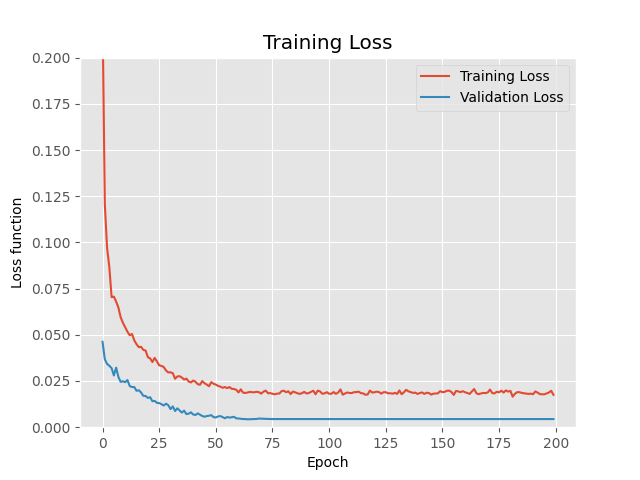
\includegraphics[width=0.7\textwidth]{resources/images/mse-finalarch.png}
    \caption{Mean squared error on the validation set}
    \label{fig:nn-validation-error-curve}
\end{figure}

Overfitting is not likely, because as can be seen in Figure \ref{fig:nn-validation-error-curve}, the validation error never increases significantly after a given amount of learning epochs, while the training error is still decreasing. An example of such obvious overfitting is shown in Figure \ref{fig:overfitting}.

\begin{figure}[h]
    \centering
    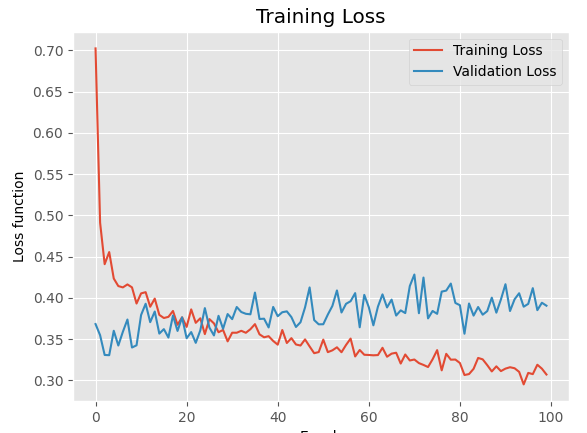
\includegraphics[width=0.6\textwidth]{resources/images/overfitting.png}
    \caption{An (unrelated) example of clear overfitting, the validation loss increasing after some time}
    \label{fig:overfitting}
\end{figure}

\subsubsection{Observations \label{ssec:surrogate-model-surf-observations}}

To further confirm the absence of overfitting in this result, the \texttt{view.py} file is used to browse across the multi-dimensional function, with surface plots.

These plots draw one of the outputs against two of the inputs, keeping the four other inputs constant. These constant values are summarized in Table \ref{tab:default-view-values}. Attention should be paid to the scale of the plots, as these do not start at 0.

\begin{table}[h!]
    \centering
    \begin{tabular}{|c|c|}
        \hline
        Input name & Value \\ \hline
        Capacity ratio & 1.15 \\
        Share flexibility & 0.5 \\
        Share storage & 0.25 \\
        Share wind & 0.25 \\
        Share PV & 0.25 \\
        rNTC & 0.35 \\ \hline
    \end{tabular}
    \caption{Default values for constant inputs. These are the middle of their base interval, see Table \ref{table:reference-values}}
    \label{tab:default-view-values}
\end{table}

Several surfaces are depicted in Figure \ref{fig:all-views}. The following observation are made from the latter illustrations.

\begin{figure}[h]
    \centering
    \begin{subfigure}[b]{0.49\textwidth}
        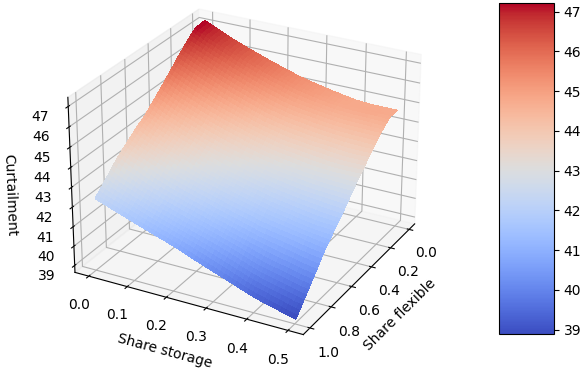
\includegraphics[width=\textwidth]{resources/images/view_1-2-0.png}
        \caption{Curtailment against share flexibility and share storage}
        \label{fig:surf-1-2-0}
    \end{subfigure}
    \hfill
    \begin{subfigure}[b]{0.49\textwidth}
        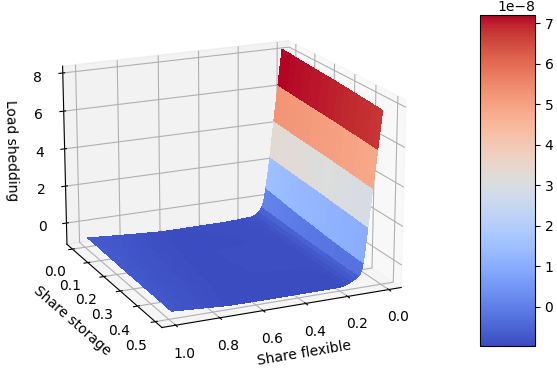
\includegraphics[width=\textwidth]{resources/images/view_1-2-1.png}
        \caption{Load shedding against share flexibility and share storage}
        \label{fig:surf-1-2-1}
    \end{subfigure}
    \hfill
    \begin{subfigure}[b]{0.49\textwidth}
        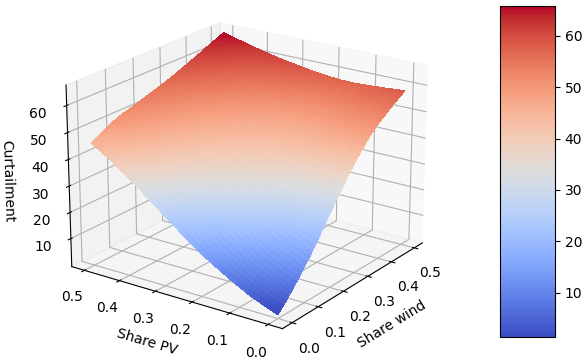
\includegraphics[width=\textwidth]{resources/images/view_3-4-0.png}
        \caption{Curtailment against share wind and share PV}
        \label{fig:surf-3-4-0}
    \end{subfigure}
    \hfill
    \begin{subfigure}[b]{0.49\textwidth}
        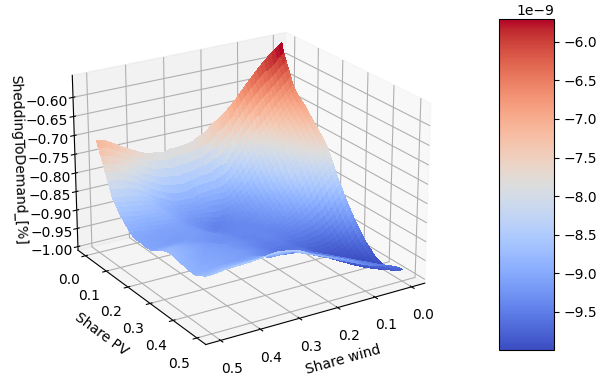
\includegraphics[width=\textwidth]{resources/images/view_3-4-1.png}
        \caption{Load shedding against share wind and share PV}
        \label{fig:surf-3-4-1}
    \end{subfigure}
    \hfill
    \begin{subfigure}[b]{0.49\textwidth}
        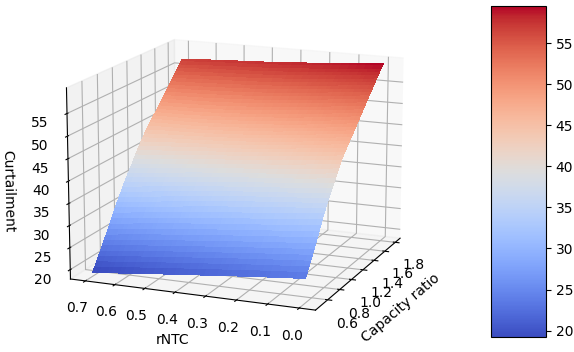
\includegraphics[width=\textwidth]{resources/images/view_0-5-0.png}
        \caption{Curtailment against capacity ratio and rNTC}
        \label{fig:surf-0-5-0}
    \end{subfigure}
    \hfill
    \begin{subfigure}[b]{0.49\textwidth}
        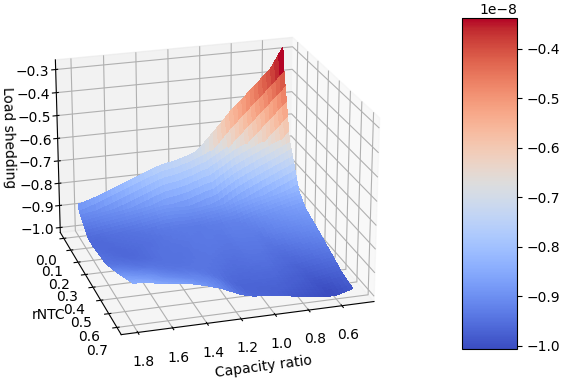
\includegraphics[width=\textwidth]{resources/images/view_0-5-1.png}
        \caption{Load shedding against capacity ratio and rNTC}
        \label{fig:surf-0-5-1}
    \end{subfigure}
    \caption{Different views of the multi-dimensional function, with four fixed inputs and two varying inputs.}
    \label{fig:all-views}
\end{figure}

\begin{itemize}
    \item Figure \ref{fig:surf-1-2-0} follows the natural intuition, as higher shares of storage units and flexible units both contribute to the reduction of the curtailment.
    \item Figure \ref{fig:surf-1-2-1} points out the crucial impact of the share of flexible units on the load shedding for small values. Naturally, when peaks in demand appear, if no unit is susceptible to be started, there is no other way than to cut the exceeding demand out.
    \item Figure \ref{fig:surf-3-4-0} also confirms the intuition, as it outlines the increase in curtailment with an increase of either share solar or share PV.
    \item Figure \ref{fig:surf-3-4-1} is the most intriguing one. First, it is noticed that the scale is the lower here. The most surprising part is that it features local minima, and that when the share PV is close to 0, the load shedding as a function of the share of wind energy is U-shaped. This phenomenon is hard to explain theoretically, the most likely cause remains a weak learning of the model.
    
    Moreover, the shape of the surface changes rapidly when changing the other constant values, therefore taking other values than disclosed in Table \ref{tab:default-view-values}, which validates the hypothesis of a weak learning.

    In comparison, the other surfaces do not move that significantly with similar change, coming down to a slight upwards or downwards shift, depending on the direction of the change, occasionnaly with a light amplitude change.
    \item Figure \ref{fig:surf-0-5-0} follows the intuition as well, but also highlights the stronger impact of the capacity ratio on the curtailment compared to the rNTC. This is not surprising, as the share of electricity import is not that huge. However, this may change dramatically depending on the country considered.
    \item Figure \ref{fig:surf-0-5-1} is interesting, as it shows that the load shedding grows when both the rNTC and capacity ratio lower. As low rNTC means little importation possible, and low capacity ratio not much margin to fulfill the demand, this actually makes sense.
\end{itemize}

% \subsection{Comparison with MEDEAS state of the art}

% Well, requires the surrogate model

% \mywarning{TODO}
\section{Integration}

\subsection{Overview}

This section describes the process of integrating the trained surrogate model into the MEDEAS model.

The MEDEAS model is built with the \href{https://vensim.com/}{Vensim} software, and is available to the public as a Vensim model file. However, the python library \href{https://pysd.readthedocs.io/en/master/index.html}{\texttt{pysd}} \cite{pysd}, focused on system dynamics simulations, is able to parse such files and run the simulations. The reasons why this will not be taken advantage of is discussed in the first subsection.

The task of integrating the surrogate model into MEDEAS is split in two smaller steps:
\begin{enumerate}
    \item \textbf{Vensim integration}, that is to make the surrogate model, available as a Tensorflow model, callable from within a Vensim model
    \item \textbf{Variable linking}, Link the input and output features of the surrogate model to the actual variables used in the MEDEAS model
\end{enumerate}

\subsection{Vensim integration}

\subsubsection{The Vensim software}

\href{https://vensim.com/}{Vensim} is a system dynamics simulation software, developped by Ventana Systems, Inc. It primarily solves the system of differential equation represented by the user-defined model, and is mainly used, according to its description, "for developing, analyzing, and packaging dynamic feedback models" \cite{vensim-website}.

Its most common application areas include \cite{wiki-vensim}:
\begin{itemize}
    \item Transportation and energy,
    \item Project management,
    \item Environment.
\end{itemize}

Vensim also comes in different distribution, such as Vensim PLE that is the free, personal learning edition. In this work, Vensim DSS is used, with an academic license.


\subsubsection{Vensim models}

Vensim provides a variety of tools to describe models, but at the end every model is an interconnection of variables, the math hiding in the connections between these. 

Vensim provides the following types of variables:
\begin{itemize}
    \item \textbf{Auxiliary variables}, that are regular variable that have no memory, that is, are independent from their value at the previous time step and are computed from every type of variable.

    For example, a $temperature$ variable that is computed from some $sunshine$ and $latitude$, that is used to compute the birth rate of $rabbits$ and $foxes$.

    \item \textbf{Constant variables}, that hold one value.
    
    For example, a mathematical constant like $\pi$.

    \item \textbf{Data variables}, or exogenous variables, whose value evolve over time but is not dependent of the model.

    For example, typical $sunshine$ data over a year.

    \item \textbf{Stock variables}, that change only over time as a function of the incoming rates, i.e., they integrates the rates.

    For example, the population of some species at a given time.

    \item \textbf{Rate variables}, or flows, that directly impact the Stock variables. 

    For example, the birth or death rate of some population at a given time.
\end{itemize}

The connections between the variables are virtually done by arrows. The only practical use of arrows is to make the variable at the origin appear in the selection of variables in the variable equation screen for the variable pointed by the arrow. But obviously they are of great utility in terms of visualization of the model.

An example of a Vensim model is depicted on Figure \ref{fig:vensim-model-example}.

\begin{figure}[h!]
    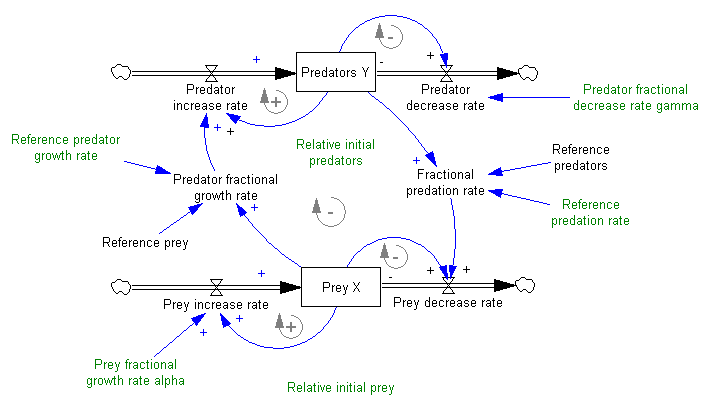
\includegraphics[width=0.9\textwidth]{resources/images/vensim-model-example.png}
    \caption{An example model in Vensim: Lotka-Volterra predator-prey model.}
    \label{fig:vensim-model-example}
\end{figure}

\subsubsection{Vensim external functions}

This specific feature of the Vensim software is evidently of great interest for this work. It enables the user to provide and use any arbitrary function in Vensim models and simulations.

To do so, the user needs to provide a dynamically linked library (DLL), packaged as a \texttt{dll} file, then provide its path in Vensim. These files are Windows specific (as Linux uses \texttt{so} files and macOS \texttt{dylib}), hence they have to be handled as such.

Dynamically linked libraries are pieces of compiled code that can be loaded at runtime by another program. User-defined functions necessarily need to be loaded at runtime, as the software cannot know them in advance. These are typically compiled from the C or C++ programming language. In this work, C++ has been chosen, as the library to load and call Tensorflow models that will be used is written in that language.

To be able to integrate the user-defined functions in its simulation environment, the user's library is expected to provide some functions, that are part of some interface that the Vensim software knows and can communicate with. This interface comprises of a set of functions that is described on Table \ref{table:vensim-interface}.
\begin{table}[h]
    \centering
    \begin{tabular}{|m{4.1cm}|m{12cm}|}
        \hline
        Function name & Description \\ \hline
        \texttt{version\_info} & Provide information about the Vensim version this library has been built for \\
        \texttt{set\_gv} & Utility to set the global variable that depend on the Vensim simulation environment \\
        \texttt{user\_definition} & Provide a way to get all the necessary information about each user-defined function, mostly their names, number of arguments and a identifier code \\
        \texttt{simulation\_setup} & This function is called by Vensim on simulation startup, allowing the library to do some preparative work if needed, such as allocating memory \\
        \texttt{simulation\_shutdown} & Same as \texttt{simulation\_setup}, but on simulation shutdown \\
        \texttt{vensim\_external} & This function is expected to, given an array of input arguments, their number and a function code, call the function associated to that code and write its return value into the first input argument.\\
        \hline
    \end{tabular}
    \caption{Description of the mandatory functions that a Vensim user library has to provide}
    \label{table:vensim-interface}
\end{table}

Luckily, %I'm not afraid of the dark
Vensim DSS ships with an example of such a library. As this file is not publicly disclosed, caution should be paid to keeping the library code private---actually, the external function capability is only available in Vensim DSS.

In the implementation of the library, this file was copied then adapted, as suggested in Vensim's documentation.

\subsubsection{Vensim subscripts}

This feature of Vensim is advertised as one of its most powerful tools. These allow to subscript variables appearing in the equations and perform operations across subscripted values if needed. For example, it enables to set predators and preys initial populations and reproduction parameters for several environments, and run them all at once. 

Importantly, MEDEAS use subscripts to run several simulations in parallel called scenarios. Therefore, one needs to edit the subscript properties in order to manage the scenario that will be run and displayed.

\subsubsection{Calling a Tensorflow model}

In consequence, it is necessary to invoke our model, presented to as a Tensorflow model, from the C or C++ language.

In order to do so, one basically needs two things:
\begin{itemize}
    \item the model in question, saved in a directory from the Tensorflow python API.
    \item the Tensorflow library, which is another DLL, to perform the actual computations from C/C++.
\end{itemize}

The complicated part being the linking between the two. In order to do so, the \href{https://serizba.github.io/cppflow/}{Cppflow} tool is used. It serves as an intermediary layer between C++ and the Tensorflow model. This tool is not available in C, this is the primary reason why the library is implemented in C++.

The main purpose of Cppflow is precisely to run Tensorflow models from C++, and to achieve this it provides user-friendly functions for loading models and making predictions using input data.

To ensure proper linkage between the library code and the two tools it utilizes—Tensorflow DLL and CppFlow—an appropriate linking strategy is necessary. To facilitate this, Makefiles were crafted using the GNU \texttt{make} utility for streamlined compilation\footnote{Previously, a program calling a Tensorflow model was created, but this did not worked from the DLL. Then, a workaround was developed using a worker process (a seperate program) and Windows' tools for interprocess communication. Later, it was discovered that the issue with calling Tensorflow stemmed from errors in linker arguments during library compilation. Once these linker issues were resolved, the need for the worker process workaround became redundant.}.

On this, one thing is to be remembered: some code may compile and link successfully, but one also has to link properly the path to the DLL you linked to, that is, not only to the compiler.

% \subsubsection{A small detour...}

% At some time in the library developpement process, it was successfully managed to produce a standalone program loading the Tensorflow model, and calling it on some inputs, but this was not the case for the library, that was able to compile and link, but not to find the DLL, once called from Vensim.

% It has been thought it may not be possible, so a workaround was implemented.

% The idea was thus to make the library communicate with another program, that would be launched as a separate process. The library would thus start the other program as an external process, that will be waiting for computation queries, on simulation setup, and end it on simulation shutdown. Then, when the model is called from the library, it sends the input to that other process, which calls the model, and sends back the output to the library, that can return.

% As previously mentioned, DLL are specific to Windows, so the process management and inter-process commication had to be done in that context.

% \subsubsection{And a fix}

% But during some more testing, and adapting of \texttt{Makefile}s, the mistake was discovered: the compilation command used to produce the library missed the indication of the path to the DLL.

% With that fixed, the library can directly use the Cppflow utilities, what greatly simplifies its architecture and code. The simulation setup loads the model, the model calls use it, and finally the simulation shutdown routine frees it.

\subsection{The pysd option}

As previously introced, the \texttt{pysd} python library can read and run Vensim model files. Of course, as the surrogate model is primarily defined in that language, one would deduce that its integration would be easier that way.

Though not explored in this work, integrating the surrogate model through \texttt{pysd} is expected to be relatively straightforward. Using the library loading functionality, a python module representing the simulation can be obtained. This module is then loaded with \texttt{pysd} to run the simulation. The linking can thus be done by editing the module file directly, and inserting the call to the model at the appropriate place. 

However, this approach was not selected. Although contemplated later in the project, after the integration into Vensim had been implemented, the main argument is the convenience of the resulting model. If the model combination was made available sa python module, it would be much harder for external people to edit the original MEDEAS model from Vensim, then run the modified version while keeping the surrogate model integrated. The editor would have to manually re-insert the surrogate model into the python module, that also have to be recreated.

Keeping the surrogate model available as a Vensim external function is therefore a significant benefit for the further improvements of the model, as it enables edits to be made to MEDEAS independently of the surrogate model.

Another update has to be mentionned here. In facts, J. Paris had trouble making the MEDEAS model run successfully with the integrated surrogate model had contact with the MEDEAS developping team, that advised to wait for the release of a update of the MEDEAS port to python, making use of \texttt{pysd} and expected to be more stable and convenient. The main issue was that she were to leave before the anticipated release date, such that it was not acheivable.

This newer Python port with \texttt{pysd} might ultimately render direct integration in Python more portable and convenient. This would offer the same advantage as the Vensim external function. Still, this function was created and finished before learning the future availability of the new python port.

\subsection{Variable linking}

In its underlying workings, the MEDEAS model does not directly employ all the variables that appear in our surrogate model. This necessitates establishing connections between the two.

Fortunately, many of the desired values bear a close relationship to existing variables within the MEDEAS energy module, so these links are expected to be as simple as linear rescalings or combinations.

The input variables, that are summarized on Table \ref{table:reference-values}, do not map directly to already existing variables in the MEDEAS model. Thus, some mappings have to be made between the inputs and outputs of the surrogate model, the Dispa-SET side, and the MEDEAS side.

This work has been done with the help of Jade Paris, a student making her master's stage thesis on this specific topic as well.

\subsubsection{Variables available in MEDEAS}

The first step in this process is to list relevant variable present in MEDEAS, that will have to be exploited in order to draw the connections.

These variable are listed on Table \ref{tab:medeas-vars}.

\begin{table}[h]
    \centering
    \begin{tabular}{|p{5cm}|p{5cm}|p{1cm}|p{4cm}|} \hline 
    MEDEAS variable name &  Description & Unit & Notation \\ \hline
     FE elec generation from solar PV TWh & Total yearly production from solar photovoltaic units & TWh & $Generation_{PV}$\\ \hline 
     Total FE Elec demand TWh & Yearly total electricity demand & TWh & $Demand_{tot}$ \\ \hline 
     FE Elec generation from offshore wind TWh & Total yearly production from offshore wind turbines & TWh & $Generation_{wind-offshore}$ \\ \hline 
     FE Elec generation from onshore wind TWh & Total yearly production from onshore wind turbines & TWh & $Generation_{wind-onshore}$ \\ \hline 
     Total capacity elec storage TW & Total power output of storage units & TW & $Storage_{tot}$ \\ \hline 
     Total FE Elec genetaion TWh EU & Total yearly electricity production from all units & TWh & $Generation_{tot}$ \\ \hline 
     new capacity installed growth rate RES elec & Yearly growth rate of the electric network capacity & [$\cdot$] & $Growth_{capacity}$ \\ \hline
    \end{tabular}
    \caption{Relevant variable in MEDEAS}
    \label{tab:medeas-vars}
\end{table}

Unfortunately, some values are not present at all in MEDEAS, so that they can't be deduced from the model as is. But as these are mandatory to run the model, a value has to be provided imperatively. In this case, a constant value will be set.

These parameters have been introduced into MEDEAS, and their potential impact on the results must be evaluated. That is, as these may have an influence on the results, this influence will have to be assessed.

\subsubsection{Linkings}

The equations linking the input variables from the surrogate model to the MEDEAS variables are provided in Table \ref{tab:linking-equations}.

\begin{table}[h]
    \centering
    \begin{tabular}{|m{3.6cm}|c|}
    \hline 
    Input variable (from surrogate model) & Linking equation \\ \hline
    $share_{PV}$ & $share_{PV}=\dfrac{Generation_{PV}}{Demand_{tot}}$ \\ \hline 
    $share_{wind}$ & $share_{wind}=\dfrac{Generation_{wind-onshore} + Generation_{wind-offshore}}{Demand_{tot}}$ \\ \hline 
    $share_{flex}$ & $share_{flex}=40\%$ \\ \hline 
    $share_{storage}$ & $share_{storage}=\dfrac{Storage_{tot}}{Demand_{tot}}\times 365\times 24$ \\ \hline 
    $Capacity_{ratio}$ & $Capacity_{ratio}=\dfrac{Generation_{tot}}{Demand_{tot}}$ \\ \hline 
    $rNTC$ & $rNTC= Growth_{capacity}$ \\ \hline 
    \end{tabular}
    \caption{Variable linking equations. The left-hand side are Dispa-SET variables, and right-hand side MEDEAS variables.}
    \label{tab:linking-equations}
\end{table}

These connections must be implemented within the Vensim model, or incorporated directly into the computation when utilizing the python version of MEDEAS.
\section{Results analysis}

\subsection{Overview}

This sections targets at describing the results observed when running the MEDEAS model integrating the created surrogate model, and to compare these with the previous results.

This comparison has to be made over the different scenarios that are defined in MEDEAS, that differ for the most part by the evolution of the electricity production mix. These scenarios were detailed in Section \ref{section:medeas-scenarios}. To simplify the analysis, only two of them are shown, BAU and OLT, as the MLT lies somewhere in between of them without adding valuable insights.

\subsection{Electricity production}

The electricity productions from the different considered VRES are the most relevant ones to consider. The comparison the values from runs with MEDEAS, to runs of the integrated MEDEAS + Dispa-SET model is made to highlight the change brought by the integration of Dispa-SET.

To make this comparison, four runs are needed, default MEDEAS and modified MEDEAS, integrating the Dispa-SET surrogate model, both with BAU and OLT scenarios.

\subsubsection{Photovoltaic units}

The photovoltaic electricity production predictions from the four runs are shown on Figure \ref{fig:electricity-production-PV}.

\begin{figure}[h]
    \centering
    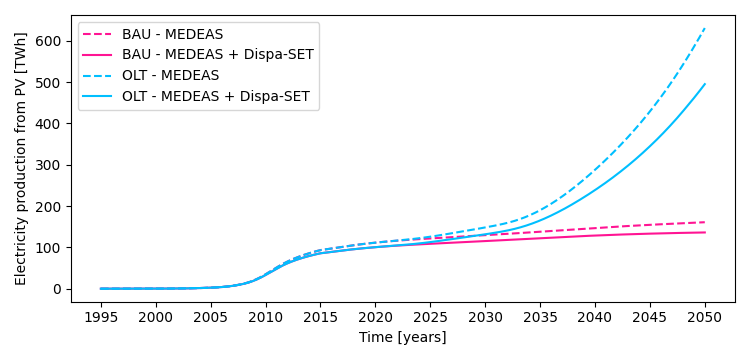
\includegraphics[width=0.8\textwidth]{resources/images/electricity-production_PV.png}
    \caption{Electricity production predictions from photovoltaic units}
    \label{fig:electricity-production-PV}
\end{figure}

We can observe that modified MEDEAS predicts a lower amount of PV energy relatively to default MEDEAS, for both scenarios. In OLT, the difference increases with the production, like if a linear factor had been applied.

\subsubsection{Onshore wind}

Figure \ref{fig:electricity-production-onshore} depicts the different predictions of the onshore wind production.

\begin{figure}[h]
    \centering
    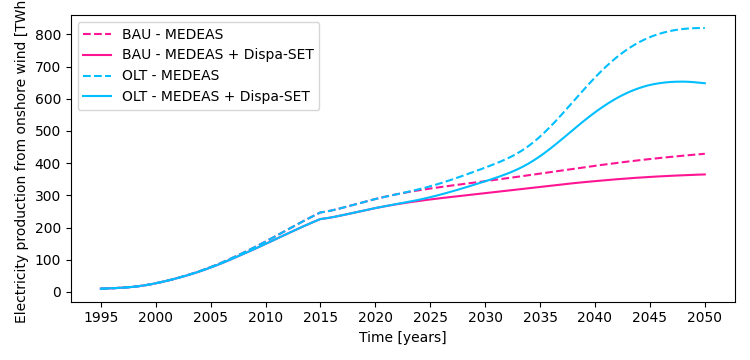
\includegraphics[width=0.8\textwidth]{resources/images/electricity-production-onshore.png}
    \caption{Electricity production predictions from onshore wind units}
    \label{fig:electricity-production-onshore}
\end{figure}

In a similar fashion to the PV production, modified MEDEAS outputs what looks like a scaled version of the default MEDEAS output. However in this case, a maximum is observed around 2050 in the OLT scenario with default MEDEAS, but this maximum is slightly moved to around 2050 when using modified MEDEAS. 

\subsubsection{Offshore wind}

Predictions of the offshore wind electricity production in the four considered cases are illustrated on Figure \ref{fig:electricity-production-offshore}.

\begin{figure}[h]
    \centering
    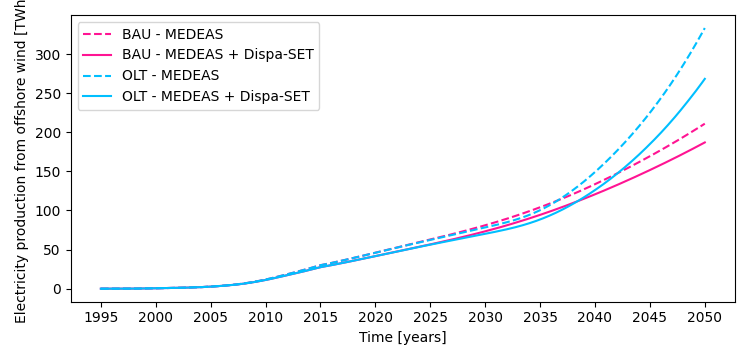
\includegraphics[width=0.8\textwidth]{resources/images/electricity-production-offshore.png}
    \caption{Electricity production predictions from offshore wind units}
    \label{fig:electricity-production-offshore}
\end{figure}

Offshore wind electricity results follows the trend observed previously, that is, the modified model predicting a smaller amount of electricity and overall as well as a larger production decrease in OLT.

\subsubsection{Hydroelectricity}

Figure \ref{fig:electricity-production-hydro} displays the outputs of the four cases for hydroelectricity production.

\begin{figure}[h]
    \centering
    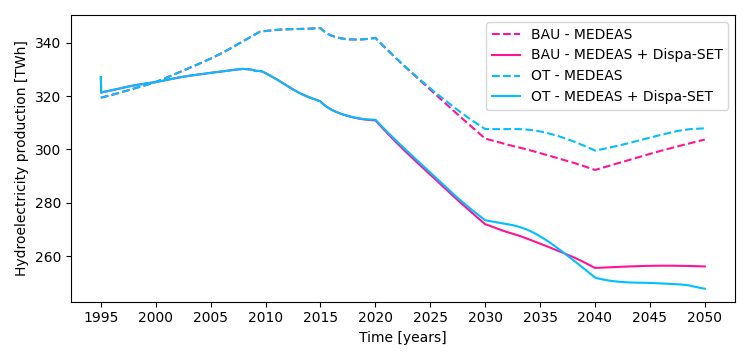
\includegraphics[width=0.8\textwidth]{resources/images/electricity-production-hydro.png}
    \caption{Electricity production predictions from hydroelectric units}
    \label{fig:electricity-production-hydro}
\end{figure}

Contrary to the previous results, where the results are grouped by scenario, that is, the shape of the curve is dictated by the scenario then is slightly changed by the model, these outcomes are grouped by model. The outputs of modified MEDEAS for BAU and OLT are close to each other, and both are very distinct from the outputs of default MEDEAS.

This phenomenon can be explained by the fact that hydroelectricity is not favored by Dispa-SET, therefore these units are avoided when possible, hence leading to a smaller use. This may be due to the geographical constraints these units are suject to, limiting their growth are there is no spot to build new units.

These are also linked to pumped hydro-storage units, as there may be such a unit build on a river. On average, the unit produces the amount of electricty dictated by the river's flow, but the total energy produced over a set period is dependent on the specific dispatch of that unit, used as a tool to manoeuvre the electricity network.

\subsubsection{Electricity mix}

Figure \ref{fig:electricity-mixes} shows the different prediction for the electricity mix in 2050.

\begin{figure}[h]
    \centering
    \begin{subfigure}{0.34\textwidth}
        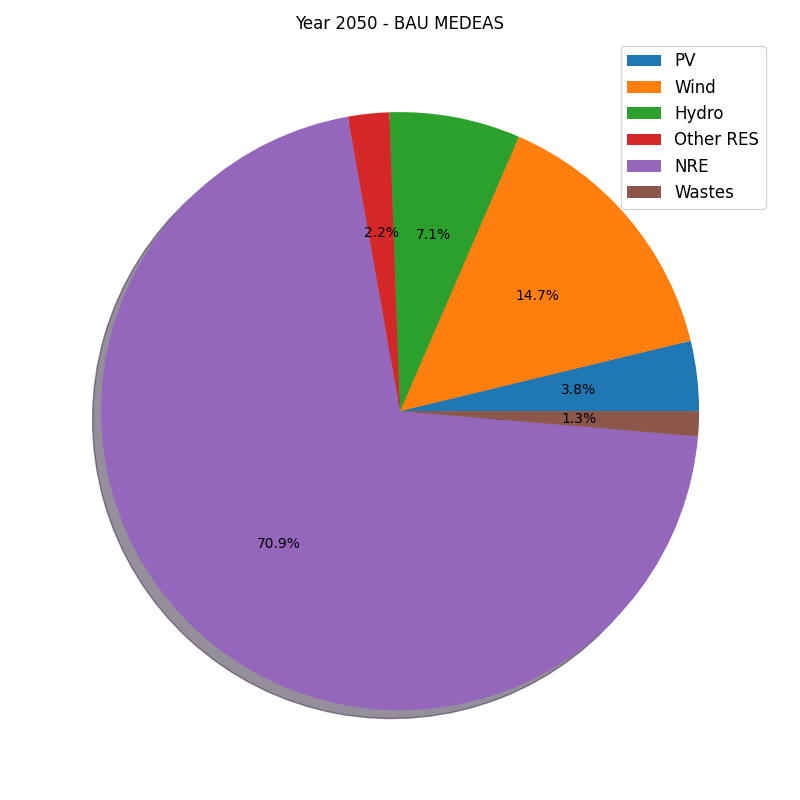
\includegraphics[width=\textwidth]{resources/images/electricity-mix-BAU-default.png}
        \caption{BAU with default MEDEAS}
        \label{fig:electricity-mix-BAU-def}
    \end{subfigure}
    \begin{subfigure}{0.34\textwidth}
        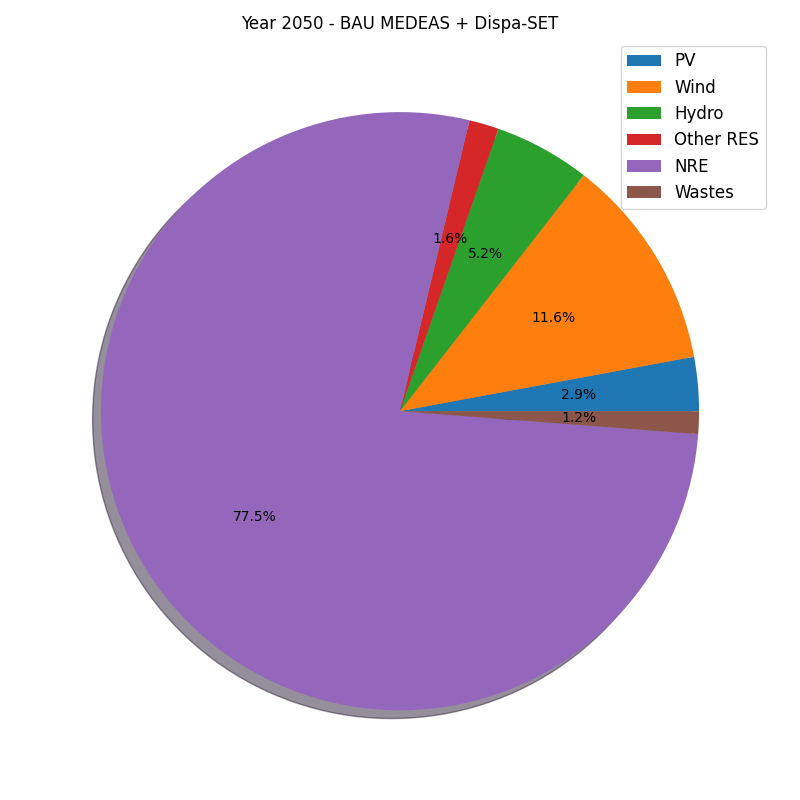
\includegraphics[width=\textwidth]{resources/images/electricity-mix-BAU-dispa.png}
        \caption{BAU with modified MEDEAS}
        \label{fig:electricity-mix-BAU-dispa}
    \end{subfigure}
    \hfill
    \begin{subfigure}{0.34\textwidth}
        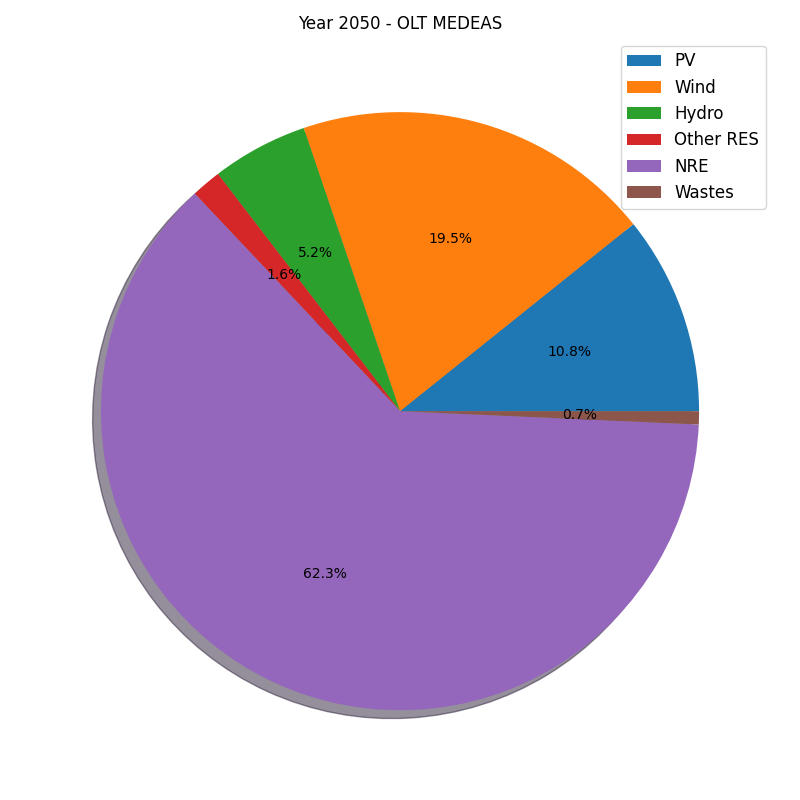
\includegraphics[width=\textwidth]{resources/images/electricity-mix-OLT-default.png}
        \caption{OLT with default MEDEAS}
        \label{fig:electricity-mix-OLT-def}
    \end{subfigure}
    \begin{subfigure}{0.34\textwidth}
        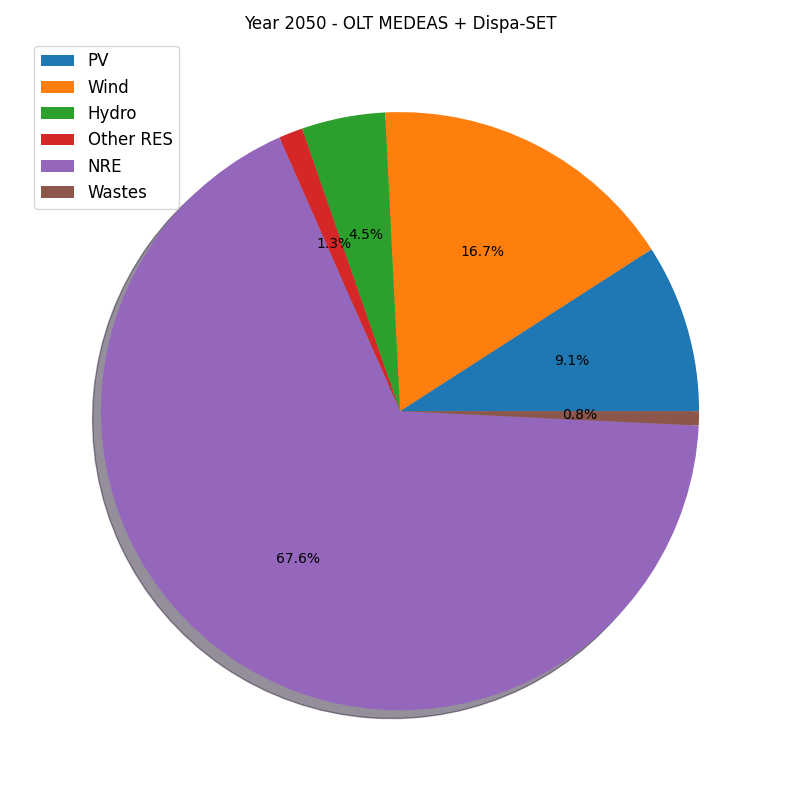
\includegraphics[width=\textwidth]{resources/images/electricity-mix-OLT-dispa.png}
        \caption{OLT with modified MEDEAS}
        \label{fig:electricity-mix-OLT-dispa}
    \end{subfigure}
    \caption{Electricity mix projection in 2050 for the four considered cases}
    \label{fig:electricity-mixes}
\end{figure}

Similarly to the previous observation, that showed lower amounts of production from VRES, the predicted share of VRES in the mix are lower in the modified version of MEDEAS.

The most intriguing change is the lower share of hydroelectricity in OLT compared to BAU, for both default and modified MEDEAS. The most likely cause for this that the total production is larger, hence as there is no growth in hydroelectricity generation, the share is reduced. 

\subsection{Curtailment}

As the surrogate model explicitly outputs the curtailment, this variable can then be plotted over a run of the modified MEDEAS. The results obtained for both scenarios are given on Figure \ref{fig:electricity-production-curtailed}.

\begin{figure}[h]
    \centering
    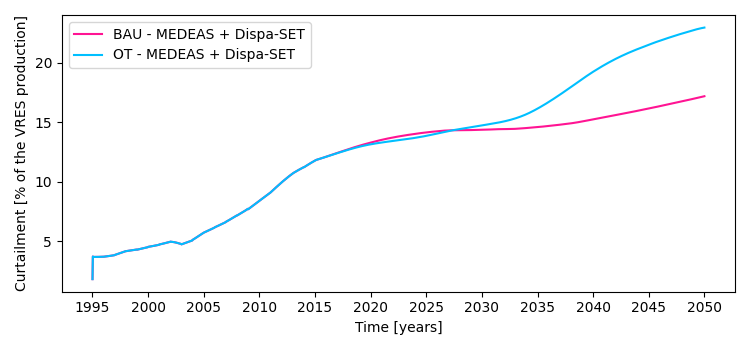
\includegraphics[width=0.9\textwidth]{resources/images/electricity-production-curtailed.png}
    \caption{Curtailment prediction of the modified MEDEAS for both scenarios}
    \label{fig:electricity-production-curtailed}
\end{figure}

We can observe from Figure \ref{fig:electricity-production-curtailed} that the OLT scenarios suffers from higher proportions of curtailment, with an higher growth rate, than in the BAU scenario. However, this increase rate looks stable.

It may be concluded that curtailment is inevitable, nonetheless every option has not been covered. For example, the distinction between different types of storage units based on the storage capacity to power output ratio has not been made. As storage facilities have a massive influence on curtailment, a more accurate modelling of these may be insightful.

\subsection{Discussion}

The figure that have been presented all yield the same conclusion: integrating the surrogate model, i.e. taking power systems constraints into account, leads to a decrease in electricity produciton from VRES. This outcome is somewhat unexpected, as the consideration of the increasing part of curtailment is symptomatic of greater quantities of wasted energy.

\subsection{Future work}

In this work, the core mechanisms for the integration have been implemented. Therefore, the most interesting contributions lie in the accuracy of surrogate model and in the quality of choice of variable. Six inputs and two outputs have been employed, but they may be improved, for example adding one input to take into account different kinds of storage facilities.

Moreover, the links drawn between the surrogate model and MEDEAS are not complete, e.g. the share of flexible units and the rNTC inputs were given as constants. First, evaluating the impact of their values on the results would be valueable. These could also be added, alongside with meaningful relations, to the MEDEAS model.


% Tools have been made to automate the creation of a dataset, including sampling and running the model; and the training of the surrogate model, using machine learning methods. The integration of the model into Vensim 
\section{Conclusion}

The goal of this thesis was to incorporate more precise flexibility constraints, evaluated through the Dispa-SET model, into an IAM, MEDEAS using a surrogate model integration strategy. This approach has been successfully implemented with an adequate choice of input and output variables.

Then, the resulting modified version of MEDEAS has been run and observations have been made. In particular, they predicted lower shares of VRES in both optimal effort and business as usual scenarios.

In the process, a database of simulations has been created on points generated through latin hypercube sampling. The complete workflow has been automated and run on a cluster.

Once the database was available, it served as the starting point to train the surrogate model. The best method was selected after several had been reviewed. Although neural networks showed the best performance, XGBoost, among gradient boosting techniques, is still highly competitive.

Finally, the linking of the model to MEDEAS has been performed, by creating an external function in Vensim, in which it is described. With the contribution of J. Paris, the model was inserted in the python version of MEDEAS, and the connections have been drawn between that surrogate model and the MEDEAS variables.

\subsection{Future work}

In this work, the core mechanisms for the integration have been implemented. Therefore, the most interesting contributions lie in the accuracy of surrogate model and in the quality of choice of variable. Six inputs and two outputs have been employed, however these choices can be refined to enhence the accuracy. For example adding one input to take into account different kinds of storage facilities.

Additionally, certain links between the surrogate model and MEDEAS have not been established, e.g. the share of flexible units and the rNTC inputs were given as constants. Evaluating the impact of their values on the results would bring valueable information. Moreover, relations could be developed and incorporated into the MEDEAS model for these variables.


\nocite{*}


\settocbibname{Bibliography}
\printbibliography[heading=bibintoc]

\setcounter{tocdepth}{0}
\setcounter{secnumdepth}{0}

\addtocounter{section}{1}
\section*{Annex A: scripts and code}

This annex documents briefly the roles of each scripts and code files.

\subsection*{Data generation}

See Table \ref{tab:annex-files-datagen}.

\begin{table}[h]
    \centering
    \begin{tabular}{|p{0.21\textwidth}|p{0.75\textwidth}|}
        \hline
        File name & Description \\ \hline
        \texttt{config.py} & Holds high level specification of the dataset to be created, such as the number of samples, the LHS strategy, and output files names. \\
        \texttt{read\_results.py} & Fetches the results from simulation directories, either one by one or all at once. \\
        \texttt{reference.py} & Runs the reference simulation and serializes the results in a json file. \\
        \texttt{sampling.py} & \texttt{--sample-only}: only run the LHS and store the samples in a CSV file. \texttt{--prepare-one idx}: prepares the simulation directory for one sample given its index. With no arguments, runs LHS and prepare all the simulation directories. \\
        \texttt{utils\_francois.py} & Stores the modified version of the \texttt{adjust\_capacity} function of Dispa-SET. \\ \hline
        \texttt{launch-job-series} \texttt{.sh} & Submits a series of simulation jobs, and a job that will submit the following series with the current one as a dependency. If the series index given as argument is too high, exits. \\
        \texttt{launch-reference-} \texttt{job.sh} & Submits the reference job. \\
        \texttt{launch-simulation-} \texttt{jobs.sh} & Submits the jobs required to run a simulation from a series. It takes the series index as an argument and the number in that series from SLURM environment variables. Uses \texttt{sampling.py --prepare-one}, GAMS and \texttt{read\_results.py} successively. \\
        \texttt{main.sh} & Starts all the scripts in the right order in order to produce a dataset. Runs the reference simulation, the sampling, prepends the header to the dataset file (as CSV), and starts the first series. \\ \hline
    \end{tabular}
    \caption{Description of the data-generation files}
    \label{tab:annex-files-datagen}
\end{table}

\subsection*{Neural network}

See Table \ref{tab:annex-files-nn}.

\begin{table}[h]
    \centering
    \begin{tabular}{|p{0.21\textwidth}|p{0.75\textwidth}|}
        \hline
        File name & Description \\ \hline
        \texttt{config.py} & Holds the configuration of the network to be trained, name, data to use, inputs and outputs. \\
        \texttt{model.py} & Holds the description of the model to be trained, via the \texttt{build\_model} function. \\
        \texttt{train.py} & Executes the tuner search for the best model and training of that best model. \\
        \texttt{view.py} & Holds different utilities to view the results of some model and its performances. Use \texttt{view.py --surface <in1> <in2> <out>} to create a 3d surface of the out-th output depending on the in1 and in2-th inputs. The other inputs are constant and parameterizable with sliders. \\
        \hline
    \end{tabular}
    \caption{Description of the files for the neural network part.}
    \label{tab:annex-files-nn}
\end{table}

\subsection*{Integration}

See Table \ref{tab:annex-files-integration}.

\begin{table}[h]
    \centering
    \begin{tabular}{|p{0.21\textwidth}|p{0.75\textwidth}|}
        \hline
        File name & Description \\ \hline
        \texttt{external.h} & Header file for \texttt{external.cpp}. \\
        \texttt{external.cpp} & Main source file for the library. \\
        \texttt{main.cpp} & Code for running a test program. \\
        \texttt{Makefile} & GNU make file for automating compilation. \\
        \texttt{tensorflow.dll} & Tensorflow library file for Windows, can be downloaded from \href{https://www.tensorflow.org/install/lang_c}{here}. \\
        \hline
    \end{tabular}
    \caption{Description of the integration files.}
    \label{tab:annex-files-integration}
\end{table}



\end{document}